\documentclass[a4paper,12pt]{article}

% Input encoding
% This is commented out because lualatex automatically understands UTF-8 and it
% might not only be redundant, but also can cause programs
%\usepackage[utf8]{inputenc}
% Font encoding
\usepackage[T1]{fontenc}
% Autogenerated text, the option is for it to be inserted in the right language
\usepackage[english]{babel}
\usepackage{graphicx}
% Setting margin between text and document border
\usepackage[margin=2cm]{geometry}
% Necessary math commands
\usepackage{mathtools}
% Math symbols
\usepackage{amssymb}
% Enabling the usage of [H] in the figure environment
\usepackage{float}
% Using subfigures
\usepackage{subfigure}
% Multiple columns
\usepackage{multicol}
% Various physics notations
\usepackage{physics}

% Need to look into what these do.
%\usepackage{grffile}
%\usepackage{longtable}
%\usepackage{wrapfig}
%\usepackage{rotating}
%\usepackage[normalem]{ulem}
%\usepackage{textcomp}
%\usepackage{capt-of}

% Feynman diagrams
\usepackage{tikz-feynman}
% Feynman slash notation
\usepackage{slashed}
% Proper quotes, mostly used in references
\usepackage{csquotes}
% Bibliography management
\usepackage[backend=biber,sorting=none]{biblatex}
% Bibliography database to use
\addbibresource{../TFM.bib}

% Putting hyperlinks, like those from the index to the section it's pointing to,
% but can also point to an equation from within the body of text
\usepackage{hyperref}
% Configuring hyperref so that hyperlinks are highlighted
\hypersetup{
colorlinks=true,
linkcolor=blue,
filecolor=magenta,
urlcolor=cyan,
}

\author{Agustín Matías Galante Cerviño}
\date{\today}
\title{Notes on ``The scotogenic model of neutrino masses and dark matter in warped extra dimensions''}
\hypersetup{
pdfauthor={Agustín Matías Galante Cerviño},
pdftitle={Notes on ``The scotogenic model of neutrino masses and dark matter in warped extra dimensions''},
pdfkeywords={},
pdfsubject={},
pdfcreator={},
pdflang={English}
}

% Using macros to shorthand some commands
\newcommand{\me}{\mathrm{e}}
\newcommand{\md}{\mathrm{d}}
\newcommand{\mi}{\mathrm{i}}
\newcommand{\hc}{\mathrm{H.c.}}
\newcommand{\Lagr}{\mathcal{L}}
\newcommand{\eff}{\mathrm{eff}}
\newcommand{\IR}{\mathrm{IR}}
\newcommand{\UV}{\mathrm{UV}}
\newcommand{\bulk}{\mathrm{bulk}}

\begin{document}

\maketitle
\tableofcontents
\clearpage
\section{Summary}
\label{sec:summary}
This thesis has, as a subject of study, models in theories with extra dimensions in which neutrinos
acquire masses through loops, which also contain a dark matter candidate. It will include a
calculation of the abundance of dark matter, (for example, from fermionic singlets in the scotogenic
model) and an analysis of the phenomenological consequences.

Since both the extra dimension and scotogenic models have been covered extensively in literature,
this thesis will only really introduce concepts without delving too deep into them, referencing
literature along the way. Main focus ought to be on calculating the abundance of this dark matter
candidate, an analysis of the phenomenological consequences and parameter space constraints.

\section{Preamble and terminology}
\label{sec:preamble}
\begin{itemize}
\item Note that by using upper case letters when referring to fields
\((L_L, \Phi)\), we are actually referring to gauge multiplets (unless stated otherwise, or in
section \ref{sec:kk}), so
\begin{equation}
L_{L, i} = \begin{pmatrix} \nu_{L,i} \\ l_{L,i} \end{pmatrix} \quad \Phi
= \begin{pmatrix} \phi^+ \\
\phi^0 \end{pmatrix} \quad \widetilde{\Phi} = \mi \sigma_2 \Phi^* = \begin{pmatrix}
\phi^{0*} \\
-\phi^{-} \end{pmatrix}
\end{equation}

Sub-index L indicates that they're left-handed (LH) fields, i and j are generational indices.

\item A regular (scalar, for simplicity) field destroys a particle at position x and creates
an antiparticle at the same position. The complex conjugate of a field creates a particle
and destroys an antiparticle. Furthermore, complex conjugate fields have the opposite
quantum numbers, so
\begin{equation}
(\phi^{+})^{*} = \phi^-
\end{equation}
has opposite electric charge, as well as opposite weak hypercharge and weak isospin, in the case of the Higgs.

\item Remember that boundary conditions are indeed physical for most cases, except for when one
has boundary conditions at infinity, or periodic conditions over an infinite interval.

\item Feynman rules of a theory are obtained by calculating the transition amplitude multiplied by i;
that is, crafting a final and initial state that can be completely contracted with the fields in
\(\Lagr_{int}\), calculating \(\bra{f}\Lagr_{int}\ket{i}\) and multiplying that by i; the resulting
Feynman rule is what's left after taking out the external line factors (fermion bispinors, polarization vectors...)

\item The lightest neutrino mass eigenstate could have no mass at all, so really the minimum amount
of Majorana right-handed (RH) fields that are to acquire mass is 2.

\item What people mean by ``integration by parts'' refers to this \cite{integrationparts}.

\item \textbf{Chirality}
I know about this by now, but a reminder doesn't hurt. A Dirac mass term is proportional to
\begin{equation}
\overline{\psi} \psi = \overline{\psi}_L \psi_R + \overline{\psi}_R \psi_L
\end{equation}
where
\begin{equation}
\psi_R = \frac{1}{2}(1 + \gamma_5) \psi \quad \psi_L = \frac{1}{2}(1 - \gamma_5) \psi
\end{equation}
and
\begin{equation}
\begin{aligned}
\overline{\psi}_R = \psi^{\dagger} \frac{1}{2}(1 + \gamma_5) \gamma^0 = \overline{\psi}
\frac{1}{2}(1 - \gamma_5) = \overline{\left(\psi_R\right)} = \overline{\left(\psi_R\right)} \\[7pt]
\overline{\psi}_L = \psi^{\dagger} \frac{1}{2}(1 - \gamma_5) \gamma^0 = \overline{\psi}
\frac{1}{2}(1 + \gamma_5) = \overline{\left(\psi_L\right)}
\end{aligned}
\end{equation}

\item \textbf{Numbers in between parenthesis}
Looks like those are just the labels for the representation of the group under which the fields
transform, since only SU(2), and U(1) are talked about here. For SU(2), the dimension of the
representation is shown, while for U(1), it's the ``charge''. With weak hypercharge, we will use
the convention \(Q = T_3 + Y\)

\item \textbf{Radiative mass}
A massless particle may acquire mass (or a massive particle change its mass),
not at tree level, but through loops with itself, given that, when renormalizing
its Lagrangian, mass terms appear. By ``radiative'', it means that there are loops involved.

\item \textbf{Weinberg operator}
A term of an effective Lagrangian, appearing on such seesaw models (actually it is their goal to end
up with this term), with mass dimension 5 (thus not renormalizable) which has the form \textbf{(this
needs checking)} \textbf{(checked, turns out Ma takes the H.c. of what I took to be the Higgs scalar doublets)}
\begin{equation}
\frac{g_{ij}}{\Lambda} \overline{L}_{L,i} \widetilde{\Phi} L^c_{L,j} \widetilde{\Phi} + \hc
= \frac{g_{ij}}{\Lambda} (\overline{\nu}_i \phi^{0*} - \overline{l}_i \phi^-)(\nu_j \phi^{0*} - l_j \phi^-) + \hc
\end{equation}

The reason for its appearance is that it is the operator with the smallest dimension that
can be added beyond the renormalizable terms of the SM Lagrangian, if formulating the SM
as an effective field theory. When EWSB occurs, this term generates a Majorana mass term
for left-handed (LH) neutrinos.

In radiative neutrino mass models, like the one considered here, we have that the ratio
\(g_{ij}/\Lambda\) is small, with \(\Lambda\) not being too big (\textasciitilde 1-100 TeV)

\item \textbf{Manifold}
Topological space locally resembling Euclidean space near each point.

\item \textbf{Orbifold}
Generalization of a manifold.

\item \textbf{3-brane}
four-dimensional subspace in \(n\)-dimensional spacetime.

\item \textbf{Graviton}
Within the scope of our study, we will consider the limit of small, linear perturbations of the metric,
in the following manner
\begin{equation}
g_{\mu \nu} \approx \eta_{\mu \nu} + h_{\mu \nu}
\end{equation}

(in 4 dimensions) with \(\eta_{\mu \nu}\) being the Minkowski metric and \(h_{\mu \nu}\) being our
graviton. This theory of quantum gravity is an effective field theory, valid below a certain
energy scale. This is a spin-2, massless particle.

\item \textbf{Graviscalar}
In five dimensions, the metric is still perturbed as above, however now we have additional
components of the metric beyond the ones belonging to the typical four dimensions.

The radion is the perturbation (\(h_{55}\), if you will) of the fifth diagonal component of the
metric \((g_{55})\). In four dimensions, this is indistinguishable from a scalar.

\item \textbf{Graviphoton or gravivector}
Same as the above, however there are additional components of the tensor aside from the one in
the diagonal which include the fifth dimension in the metric \((g_{\mu 5})\), so the perturbation
is now a massless vector field when seen in four dimensions \((h_{\mu 5})\).
\end{itemize}

\section{Neutrino masses}
\label{sec:neumass}
\subsection{Motivation}
It is perfectly possible to grant mass to neutrinos by extending the SM with Yukawa interaction terms
analogous to those used with right-handed quarks, as well as sterile, right-handed neutrinos.
However, many have taken issue with the extremely small couplings (\(<10^{-12}\)) necessary to fit
observations, strongly believing that such a disparity with analogous couplings indicates that the
mechanism involved is more complex than this extension. As a result, a myriad of models sprung up in
the past 40 years aiming to provide a more compelling way of resolving this problem.

\subsection{Seesaw models}
\label{sec:seesaw}
A family of models used to generate neutrino masses. Mostly taken from \cite{claude2015}, additional
section to chapter 14.

Let us take one family of neutrinos, however this can be applied to any number of them.
The fields from which we can build a theory are, \(\psi_L\), \(\psi_R\),
\((\psi^c)_R = 1/2 (1 + \gamma_5)\psi^c\),
\((\psi^c)_L\), as well as \(\overline{\psi}_L\), \(\overline{\psi}_R\),
\(\overline{(\psi^c)_R}\), and \(\overline{(\psi^c)_L}\). Remember that, as
the representation \textbf{2} of SU(2) is equivalent to its conjugate, we also have
to take into account the latter when adding Lorentz invariant terms to the Lagrangian,
so that is presumably why the charge conjugated fields are included. (I doubt this can
be done if parity is to be respected, doesn't a Majorana mass term violate parity? Doubt it
does, otherwise I'd see it mentioned).

They are not quite this (we're using the Weyl representation throughout this section),
\begin{equation}
\psi^c = C \psi^* = C \begin{pmatrix} \psi^*_L \\ \psi^*_R \end{pmatrix}
\end{equation}

but from the definition of the charge conjugation operator,
(this being a matrix in bispinor space, like parity, gamma matrices\ldots)
\begin{equation}
C \gamma_{\mu} C^{-1} = -(\gamma_{\mu})^T
\end{equation}

one can see that
\begin{equation}
\psi^c = \begin{pmatrix}(\psi^{c})_{L} \\
(\psi^{c})_{R} \end{pmatrix} = C \overline{\psi}^T = C \begin{pmatrix} \psi^*_R \\
\psi^*_L \end{pmatrix} = \begin{pmatrix} \mi \sigma^2 & 0 \\
0 & - \mi \sigma^2 \end{pmatrix} \begin{pmatrix} \psi_R^* \\
\psi_L^* \end{pmatrix} =\begin{pmatrix} \mi \sigma^2 \psi_R^* \\
- \mi \sigma^2 \psi_L^* \end{pmatrix}
\end{equation}

Mass terms containing these fields are the following,
\begin{equation}
M_D \overline{\psi}_R \psi_L + \frac{1}{2} M_L \overline{(\psi_L)^c} \psi_L + \frac{1}{2} M_R \overline{(\psi_R)^c} \psi_R + \hc
\end{equation}

It's important to note that Majorana mass terms (the two last ones) violate leptonic number by two units.
We also have that
\begin{equation}
(\psi^c)_L = \mi \sigma_2 \psi^*_R = (\psi_R)^c \quad (\psi^c)_R = -\mi \sigma_2 \psi^*_L = (\psi_L)^c
\end{equation}
so indeed the fundamental and its conjugate rep. are in the same term.

The kicker is that we can just include both these Dirac and Majorana mass terms in the same
Lagrangian, if our criterion for adding more terms is that they must be Lorentz invariant. For
arbitrary Dirac and Majorana mass parameters these fields are not the eigenstates of the
Hamiltonian, thus they do not generate physical, observable states. One needs to redefine the
fields,
\begin{equation}
f = \frac{1}{\sqrt{2}}(\psi_L + (\psi^c)_R) \quad F = \frac{1}{\sqrt{2}}(\psi_R + (\psi^c)_L)
\end{equation}

These are Majorana fields, since \(f^c = f\) and \(F^c = F\). Remember that, for a left-handed and
right-handed Majorana field, the bispinors are
\begin{equation}
\begin{pmatrix} \psi_L \\ \mi \sigma_2 \psi^*_L \end{pmatrix}
\quad \begin{pmatrix} \mi \sigma_2 \psi^*_R \\ \psi_R \end{pmatrix}
\end{equation}

One now gets the mass terms
\begin{equation}
M_L \overline{f}f + M_R \overline{F}F + M_D (\overline{f}F + \overline{F}f)
= (\overline{f} \: \overline{F}) \begin{pmatrix} M_L & M_D \\ M_D & M_R \end{pmatrix} \begin{pmatrix} f \\
F \end{pmatrix}
\end{equation}
(This setup laid down is what most seesaw models get at.)

This is, again, not physical, so diagonalizing this matrix, and finding eigenvalues
and eigenvectors will yield observable masses and fields. These are
\begin{equation}
\nu' = \frac{1}{\sqrt{2}}(F + f) \quad N = \frac{1}{\sqrt{2}}(F - f)
\end{equation}

Note that kinetic terms (ones with derivatives of the fields) are always diagonal in flavor,
and so they are not affected by field redefinitions, they are always diagonal
in whatever field is chosen \textbf{(need to check this)}. In the case \(M_L = M_R = 0\), we get
\begin{equation}
-M_D \overline{\nu}' \nu' + M_D \overline{N} N = M_D \overline{\nu} \nu + M_D \overline{N} N
\end{equation}
where \(\nu = \gamma_5 \nu'\), a redefinition made so that the mass remains
positive. Another case is \(M_L = 0, M_R >> M_D\), which

In the type-I seesaw, an additional Higgs-like scalar field singlet (under every group except
\(U(1)_{B-L}\)) is added in order to grant the RH neutrino a Majorana mass
term when this symmetry is spontaneously broken.

\section{Scotogenic model}
\label{sec:scm}
Generation of neutrino masses at one loop order, through the coupling at one loop of SM neutrino
flavour eigenstates with the Higgs through a Higgs copy. \cite{ma2006verifiable}

The scotogenic model consists in the generation of neutrino masses through the coupling at one loop
of neutrinos with the SM Higgs through various new particles, these being a Higgs-like scalar
doublet under \(SU(2)_{L}\), \(\eta\), and fermionic singlets, \(N_{i}\). In order to accomplish
this, an exact \(Z_2\) symmetry is introduced as well. If the Higgs potential, now containing both
the SM Higgs and this doublet, is to respect this symmetry, then the bilinear term mixing both
fields, \(\mu^{2}\Phi^{\dagger}\eta\), has to be forbidden. This term would otherwise have been able
to give neutrinos mass at tree level. Not only does this model attempt to explain the origin of
neutrino masses, but it also happens to provide a good candidate to dark matter, given that there is
a lightest stable particle that could either be the lightest \(N_{i}\) or
\(\sqrt{2} \: \mathrm{Re} \: \eta^{0}\).

In other words, it distinguishes the ``neutrinophobic'' regular Higgs doublet from the ``neutrinophilic''
\(\eta\). If \(Z_2\) is exact, the lightest (charged) RH neutrino is stable and a dark matter
candidate, Representations (of \(SU(2)_L \times U(1)_Y \times Z_{2}\)) of relevant particles are the
following; we first have the SM lepton LH doublet and RH singlet,

\begin{multicols}{2}
\begin{itemize}
\item \(L_i\) = \((\nu_i, l_i)^T\) \(\sim\) \((2, -1/2, +)\)
\item \(l^c_i\) \(\sim\) \((1, -1, +)\)
\end{itemize}
SM Higgs doublet,
\begin{itemize}
\item \(\Phi\) = \((\phi^{+}, \phi^{0})^T\) \(\sim\) \((2, 1/2, +)\)
\item \(\widetilde{\Phi}\) = \((\phi^{0*}, -\phi^{-})^T\) \(\sim\) \((2, -1/2, +)\)
\end{itemize}
%\vfill\null
%\columnbreak
new Higgs-like scalar doublet,
\begin{itemize}
\item \(\eta\) = \((\eta^{+}, \eta^{0})^T\) \(\sim\) \((2, 1/2, -)\)
\item \(\widetilde{\eta}\) = \((\eta^{0*}, -\eta^{-})^T\) \(\sim\) \((2, -1/2, -)\)
\end{itemize}
and finally, the fermionic singlets,
\begin{itemize}
\item \(N_{i}\) \(\sim\) \((1, 0, -)\).
\end{itemize}
\end{multicols}
The Yukawa interactions of this model are (all leptonic fields are taken to be LH so we drop the L sub-index)
\begin{equation}
f_{ij} \overline{L}_{i} \Phi l^c_{j} + h_{ij} \overline{L}_{i} \widetilde{\eta} N_j + \hc =
f_{ij} (\overline{\nu}_{i}\phi^{+} + \overline{l}_{i}\phi^{0}) l^c_{j} +
h_{ij} (\overline{\nu}_{i}\eta^{0*} - \overline{l}_{i}\eta^{-}) N_j + \hc
\end{equation}
and the most general Higgs potential allowed is
\begin{equation}
\begin{aligned}
V(\Phi, \eta) = m^{2}_{1} \Phi^{\dagger}\Phi + m^{2}_{2} \eta^{\dagger}\eta
+ \frac{1}{2}\lambda_{1}(\Phi^{\dagger}\Phi)^{2}
+ \frac{1}{2}\lambda_{2}(\eta^{\dagger}\eta)^{2} \\
+ \lambda_{3}(\Phi^{\dagger}\Phi)(\eta^{\dagger}\eta)
+ \lambda_{4}(\Phi^{\dagger}\eta)(\eta^{\dagger}\Phi)
+ \frac{1}{2}\lambda_{5}[(\Phi^{\dagger}\eta)^{2} + \hc]
\end{aligned}
\end{equation}
The fermionic singlets also admit a Majorana mass term,
\(\frac{1}{2}M_{i}\overline{N_{i}}^{c}N_{i}\). In the original paper, this mass was put in
by hand rather than having a dynamical origin like all the other masses.
Putting all this together allows for the loop in figure \ref{fig:scmmass1} to generate Majorana
mass terms when electroweak symmetry breaking (EWSB) takes place,
\begin{figure}[H]
\centering
\begin{tikzpicture}
\begin{feynman}
\vertex (i) {\(\nu_{i}\)};
\vertex[right=1.6cm of i] (a);
\vertex[right=2.2cm of a] (b);
\vertex[right=1.6cm of b] (f) {\(\nu_{j}\)};
\vertex[right=1.1 of a] (aux);
\vertex[above=1.65cm of aux] (c);
\vertex[above=3.3cm of a] (d) {\(\phi^0\)};
\vertex[above=3.3cm of b] (e) {\(\phi^0\)};

\diagram*{
(i) -- [plain] (a) -- [plain, edge label'=\(N_{s}\)] (b) -- [plain] (f),
(a) -- [anti charged scalar, edge label=\(\eta^{0}\)] (c) -- [anti charged scalar] (e),
(b) -- [anti charged scalar, edge label'=\(\eta^{0}\)] (c) -- [anti charged scalar] (d),
};
\end{feynman}
\end{tikzpicture}
\caption{Feynman diagram of the process responsible for giving mass to neutrinos}
\label{fig:scmmass1}
\end{figure}

\subsection{Neutrino mass matrix}
We shall now lay down the calculation for said mass matrix. Let us start with considering the
Lagrangian after EWSB, so we will take \(\Phi = (0, v)^{T}\), with \(v\) being the known
VEV of the SM Higgs. The Higgs potential detailed above becomes
\begin{equation}
\begin{aligned}
&= m^{2}_{2}(\eta^{+*} \eta^{+} + \eta^{0*} \eta^{0}) + \frac{\lambda_{2}}{2} (\eta^{+*} \eta^{+} + \eta^{0*} \eta^{0})^{2} \\
&+ \lambda_{3}v^{2}(\eta^{+*} \eta^{+} + \eta^{0*} \eta^{0}) + \lambda_{4}v^{2}\eta^{0*} \eta^{0} + \frac{1}{2}\lambda_{5}v^{2}((\eta^{0})^{2} + (\eta^{0*})^{2}) \\
&= (m^{2}_{2} + \lambda_{3}v^{2}) \eta^{+*} \eta^{+} + \frac{\lambda_{2}}{2} (\eta^{+*} \eta^{+})^{2} \\
& + v^{2}(\lambda_{3} + \lambda_{4}) \eta^{0*} \eta^{0} + \frac{\lambda_{5}v^{2}}{2}((\eta^{0})^{2} + (\eta^{0*})^{2}) + \frac{\lambda_{2}}{2} (\eta^{0*} \eta^{0})^{2} \\
& + \lambda_{2} (\eta^{+*} \eta^{+} \eta^{0*} \eta^{0})
\end{aligned}
\end{equation}
We see that, while \(\eta^{+}\)'s mass terms are obtained straightfowardly just by looking at the
potential, \(\eta^{0}\) has quadratic couplings not corresponding to a mass term, and as such
this is not the mass eigenstate. We will need to redefine this field in order to use the right
propagators in our one-loop calculation. So, we use two real fields, which are the
real and imaginary part of \(\eta^{0}\), so \(\eta^{0} = \eta^{0}_{R} + \mi \eta^{0}_{I}\)
and \(\eta^{0*} = \eta^{0}_{R} - \mi \eta^{0}_{I}\).
% Right after this, lay down the potential as a function of these fields
The masses we obtain are
\begin{equation}
\begin{aligned}
m^{2}(\eta^{\pm}) \equiv m^2_{\eta} &= m^{2}_{2} + \lambda_{3} v^{2}\\
m^{2}(\sqrt{2} \eta^{0}_{R}) \equiv m^{2}_{R} &= m^{2}_{2} + (\lambda_{3} + \lambda_{4} + \lambda_{5}) v^{2}\\
m^{2}(\sqrt{2} \eta^{0}_{I}) \equiv m^{2}_{I} &= m^{2}_{2} + (\lambda_{3} + \lambda_{4} - \lambda_{5}) v^{2}\\
\end{aligned}
\end{equation}

Having settled this matter, we shift our focus to the loop itself. After EWSB, we may ignore
the coupling to the surviving Higgs field and merely consider \(\eta^{0}_{R}\) and \(\eta^{0}_{I}\)
with their new masses, so we end up dealing with 2 \(\cdot\) \(N_{fs}\) self-energy diagrams.
This is because we have two scalar fields, and \(N_{fs}\) fermionic singlets. Now, we take
a look at how the Yukawa interactions look like with the new definitions,
\begin{equation}
\begin{aligned}
h_{ij} \overline{\nu}_{i}\eta^{0*} N_j + h_{ij} \overline{N}_{j}\eta^{0} \nu_i
= h_{ij} \overline{\nu}_{i}\eta^{0}_{R} N_j + h_{ij} \overline{N}_{j}\eta^{0}_{R} \nu_i
- \mi h_{ij} \overline{\nu}_{i}\eta^{0}_{I} N_j + \mi h_{ij} \overline{N}_{j}\eta^{0}_{I} \nu_i
\label{eq:yukscm}
\end{aligned}
\end{equation}
and we see that not much changes, aside from a relative sign and a couple of factors of i.
These latter factors will play out a critical role in the following.
\vspace{-2ex}
\begin{figure}[H]
\centering
\feynmandiagram [large, baseline=(d.base), layered layout, horizontal=b to c] {
a [particle=\(\nu_i\)] -- [fermion, momentum=\(p\)] b -- [scalar, half left, looseness=1.5, momentum=\(p-k\), edge label'=\(\eta^0_R/\eta^0_I\)] c
-- [anti fermion, half left, looseness=1.5, momentum=\(k\), edge label'=\(N_s\)] b,
c -- [anti fermion, momentum=\(p\)] d [particle=\(\nu_j\)],
};
\caption{Diagram of the resulting self-energy process after EWSB from fig. \ref{fig:scmmass1}}
\label{fig:scmmass2}
\end{figure}

Calculating the reduced amplitude through the use of the Feynman diagram in
figure \ref{fig:scmmass2} yields
\begin{equation}
\begin{aligned}
\begin{gathered}
\mi \mathcal{M} = \overline{u}_{\nu_j}(p, r)\sum_{s}\int \frac{\mu^{4-D}\md^{D}k}{(2\pi)^{D}}
\Bigg(\frac{\mi}{(p - k)^{2} - m^{2}_{R}} (\mi h_{js} P_L) \frac{\mi (\slashed{k} + M_{s})}{k^{2} - M^{2}_{s}} (\mi h_{is} P_L) \\
+ \frac{\mi}{(p - k)^{2} - m^{2}_{I}} (h_{js} P_L) \frac{\mi (\slashed{k} + M_{s})}{k^{2} - M^{2}_{s}}(h_{is} P_L)\Bigg)
u_{\nu_i}(p, r) \\
= \overline{u}_{\nu_j}(p, r) [-\mi \Sigma(p^{2})] u_{\nu_i}(p, r)
\end{gathered}
\end{aligned}
\end{equation}
with \(D = 4 - \epsilon\), \(\epsilon \rightarrow 0\) as we're using dimensional regularization. 
So the radiative correction to the neutrino propagator is this amplitude without the external line factors,
these being the neutrino bispinors,
\begin{equation}
- \mi \Sigma(p^{2}) = - P_L \sum_{s}h_{is}h_{js} \int \frac{\mu^{4-D}\md^{D}k}{(2\pi)^{D}}
\left( \frac{\mi}{(p - k)^{2} - m^{2}_{R}} \frac{\mi M_{s}}{k^{2} - M^{2}_{s}}
- \frac{\mi}{(p - k)^{2} - m^{2}_{I}} \frac{\mi M_{s}}{k^{2} - M^{2}_{s}}\right)
\end{equation}
So we see that we really only have to solve one integral, up to the mass of the scalar in the loop.
This integral is
\begin{equation}
\int \frac{\mu^{4-D}\md^{D}k}{(2\pi)^{D}} \frac{M_{s}}{[(p - k)^{2} - m^{2}_{R}][k^{2} - M^{2}_{s}]}
\end{equation}
so now we make use of Feynman parametrization,
\begin{equation}
\frac{1}{AB} = \int^1_0 \md x \: \frac{1}{(xA + (1-x)B)^2}; \quad A = (p-k)^2 - m^2_R, \quad B = k^2 - M^2_s
\end{equation}
which yields
\begin{equation}
\int \frac{\mu^{4-D}\md^{D}k}{(2\pi)^{D}}\int^1_0 \md x \: \frac{M_{s}}{[((p-k)^2 - m^2_R)x + (k^2 - M^2_s)(1-x)]^2}
\end{equation}
Now, we need to manipulate the denominator a bit,
\begin{equation}
\begin{aligned}
\begin{gathered}
((p-k)^2 - m^2_R)x + (k^2 - M^2_s)(1-x) = p^2 x + k^2 x - 2(pk)x - m^2_R x + k^2 - k^2 x - M^2_s + M^2_s x \\
= k^2 - 2(pk)x + p^2 x^2 - p^2 x^2 + p^2 x - m^2_R x - M^2_s + M^2_s x \\
= (k - px)^2 - p^2 x^2 + p^2 x - m^2_R x - M^2_s + M^2_s x \\
= (k - px)^2 - p^2 x(x-1) + M^2_s(x-1) - m^2_R x \equiv l^2 - \Delta
\end{gathered}
\end{aligned}
\end{equation}
where we defined \(l = k - px\) and \(\Delta = m^{2}_{R}x - (p^{2}x - M^{2}_{s})(1-x)\). The resulting
integral is
\begin{equation}
\begin{aligned}
\begin{gathered}
M_{s}\mu^{4-D} \int^1_0 \md x \: \int \frac{\md^{D}k}{(2\pi)^{D}} \frac{1}{(l^2 - \Delta)^2}
\end{gathered}
\end{aligned}
\end{equation}
Knowing that
\begin{equation}
\int \md^{D}k \frac{1}{(l^2 - \Delta)^N} = \mi (-1)^N \pi^{\frac{D}{2}} \frac{\Gamma(N - \frac{D}{2})}{\Gamma(N)}\Delta^{\frac{D}{2}-N}
\label{eq:intrenor}
\end{equation}
we evaluate the integral with respect to \(k\) and press on,
\begin{equation}
\begin{aligned}
\begin{gathered}
= \frac{\mi M_{s}}{(4\pi)^{D/2}}\mu^{4-D} \Gamma \left(2 - \frac{D}{2}\right) \int^{1}_{0} \md x \Delta^{D/2 - 2}\\
= \left[\Gamma\left(2 - \frac{D}{2}\right) = \Gamma\left(\frac{\epsilon}{2}\right) \approx \frac{2}{\epsilon} - \gamma_{E}; \quad \Delta^{D/2 - 1} = \Delta^{-\epsilon/2} \approx 1 - \frac{\epsilon}{2}\ln \Delta\right] =\\
= \mi M_{s} (4\pi)^{-\frac{1}{2}(4-\epsilon)}\mu^{\epsilon}\left(\frac{2}{\epsilon} - \gamma_{E}\right) \int^{1}_{0} \md x \Delta^{-\epsilon/2}\\
\approx \frac{\mi}{(4\pi)^{2}} \left(1 + \frac{\epsilon}{2}\ln 4\pi \right) (1 + \epsilon \ln \mu)
\left(\frac{2}{\epsilon} - \gamma_{E}\right) \int^{1}_{0} \md x M_{s}\left(1 - \frac{\epsilon}{2} \ln \Delta\right)\\
\approx \frac{\mi M_{s}}{(4\pi)^{2}} \left(\frac{2}{\epsilon} - \gamma_{E} + \ln 4\pi \mu^2 \right)\int^{1}_{0} \md x \left(1 - \frac{\epsilon}{2} \ln \Delta\right)\\
\approx \frac{\mi M_{s}}{(4\pi)^{2}} \left(\frac{2}{\epsilon} - \gamma_{E} + \ln 4\pi\mu^2 \right)
- \frac{\mi M_{s}}{(4\pi)^{2}} \int^{1}_{0} \md x \ln \Delta
\label{eq:massmint}
\end{gathered}
\end{aligned}
\end{equation}
Let's stop here for a second and appreciate that the divergent contribution to this correction does
not depend on the mass of the scalar, which means that the two sorts of diagrams here, each with a
different scalar and opposite sign, have their divergent parts (and other terms not depending on this mass)
cancel each other out without resorting to renormalization. Let's remember that we are attempting to
correct the mass, so this means that, if terms proportional to \(\slashed{p}\) survived, we could
safely disregard them, however they were eliminated, as being sandwiched between two identical
chirality projectors means that it doesn't contribute, since \(P_L \slashed{k} P_L = P_L P_R \slashed{k} = 0\)
because \(\{\gamma_5, \gamma^{\mu}\} = 0\). Not only that, we shall set \(p^{2} = 0\), since neutrinos are massless at tree level.
\textbf{(Is this the actual reason? I'd say so but I could use feedback)}.
\begin{equation}
\begin{aligned}
\begin{gathered}
-\frac{\mi M_{s}}{(4\pi)^{2}} \int^{1}_{0} \md x \ln (m^{2}_{R}x + M^{2}_{s}(1-x))\\
= -\frac{\mi M_{s}}{(4\pi)^{2}} \left(\frac{M^{2}_{s}\ln M^{2}_{s} - m^{2}_{R}\ln m^{2}_{R} + m^{2}_{R} - M^{2}_{s}}{M^{2}_{s} - m^{2}_{R}}\right)\\
% We need to clarify this last step.
= -\frac{\mi M_{s}}{(4\pi)^{2}} \frac{m^{2}_{R}}{m^{2}_{R} - M^{2}_{s}}\ln \frac{m^{2}_{R}}{M^{2}_{s}}
\label{eq:asss}
\end{gathered}
\end{aligned}
\end{equation}
Now, all we need to obtain the resulting correction to the mass is to do this again, but with
\(\eta^0_I\) rather than \(\eta^0_R\) as we have just done, and to sum their contributions.
The resulting mass matrix is this times i,
\begin{equation}
\begin{aligned}
\begin{gathered}
(m_{\nu})_{ij} = \sum_{s}\frac{h_{is}h_{js}M_{s}}{16\pi^{2}}\left( \frac{m^{2}_{R}}{m^{2}_{R} - M^{2}_{s}}\ln \frac{m^{2}_{R}}{M^{2}_{s}} -
\frac{m^{2}_{I}}{m^{2}_{I} - M^{2}_{s}}\ln \frac{m^{2}_{I}}{M^{2}_{s}} \right)
\label{eq:massmat}
\end{gathered}
\end{aligned}
\end{equation}

\subsection{Lepton flavor violation}
As Majorana neutrinos do not possess a global lepton flavor symmetry, charged leptons
may transmute into others violating lepton flavor number conservation. The most sought after
process is \(\mu \rightarrow e \gamma\), having very strong upper limits for its decay rate.
The effective Lagrangian describing this decay is (\cite{Beneke_2016}, page 6, eq. (10))
\begin{equation}
\begin{aligned}
\begin{gathered}
\Lagr_{l_i \rightarrow l_j \gamma} = A_R m_i \overline{l}_j \sigma^{\mu \nu}F_{\mu \nu} P_R l_i
+ A_L m_i \overline{l}_j \sigma^{\mu \nu}F_{\mu \nu} P_L l_i + \hc \\
= A_R m_i \overline{l}_{j,L} \sigma^{\mu \nu}F_{\mu \nu} l_{i,R}
+ A_L m_i \overline{l}_{j,R} \sigma^{\mu \nu}F_{\mu \nu} l_{i,L} + \hc
\end{gathered}
\end{aligned}
\end{equation}
where subindex \(i\) denotes the heavier lepton, in our case the muon.
\begin{equation}
A_R = - \frac{e(F_2 (0) - \mi F_3(0))}{4m^2_{i}}; \quad A_L = - \frac{e(F_2 (0) + \mi F_3(0))}{4m^2_{i}}
\label{eq:aral}
\end{equation}

\begin{figure}[H]
\centering
\begin{tikzpicture}
\begin{feynman}
\vertex (i) {\(l_i\)};
\vertex[right=2.5cm of i] (a);
\vertex[right=3.2cm of a] (aux1);
\vertex[above=1.6cm of aux1] (b);
\vertex[below=1.6cm of aux1] (c);
\vertex[right=1.8cm of aux1] (aux2);
\vertex[above=3.5cm of aux2] (f1) {\(\gamma\)};
\vertex[below=3.5cm of aux2] (f2) {\(l_j\)};

\diagram*{
(i) -- [fermion, momentum=\(q_1\)] (a) -- [plain, edge label=\(N_{s}\), rmomentum'=\(k-q_1\)] (c) -- [fermion, momentum=\(q_2\)] (f2),
(a) -- [charged scalar, edge label'=\(\eta^{-}\), momentum=\(k\)] (b) -- [photon, rmomentum=\(p\)] (f1),
(b) -- [charged scalar, edge label'=\(\eta^{\pm}\), momentum=\(k+p\)] (c),
};
\end{feynman}
\end{tikzpicture}
\caption{One-loop diagram responsible for \(l_i \rightarrow l_j \gamma\)}
\label{fig:egamma}
\end{figure}

The Feynman rule for the uppermost interaction in fig. \ref{fig:egamma} is \(\mi e (k - (-k - p))_{\mu} = \mi e (2k + p)_{\mu}\),
taken from \cite{Romao_2012}, page 15; even though those rules are for the SM Higgs, \(\eta\)'s covariant derivative
is identical, since their quantum numbers are the same.\footnote{Also, according to this paper, we have chosen \(\eta_e = -1\)}

The reduced amplitude for this process is (making use of dimensional regularization from the get-go)
\begin{equation}
\begin{aligned}
\mi \mathcal{M} = \varepsilon^*_{\mu}(p, \lambda) \overline{u}_{l_j} (q_2, r_2) \Bigg(\sum_s \int \frac{\mu^{4 - D}\md^D k}{(2\pi)^D} 
\frac{\mi}{k^2 - m^2_{\eta}}(\mi e (2k^{\mu} + p^{\mu}))\frac{\mi}{(k + p)^2 - m^2_{\eta}} \\
\cdot (\mi h_{js} P_L) \frac{\mi(\slashed{k} - \slashed{q_1} + M_s)}{(k-q_1)^2 - M^2_s} (\mi h_{is} P_R) \Bigg) u_{l_i} (q_1, r_1) 
\end{aligned}
\end{equation}
so the vertex integral is said amplitude without the external line factors, that is, without the charged lepton bispinors and
photon polarization vector,
\begin{equation}
\begin{aligned}
\Gamma^{\mu} = - e  P_L \sum_s h_{is} h_{js} \int \frac{\mu^{4 - D}\md^D k}{(2\pi)^D} 
\frac{(2k^{\mu} + p^{\mu})(\slashed{k} - \slashed{q_1})}{[k^2 - m^2_{\eta}][(k + p)^2 - m^2_{\eta}][(k-q_1)^2 - M^2_s]}
\end{aligned}
\end{equation}
We are going to somewhat mirror the discussion in \cite{peskshro}, chapter 6.3, beginning at page
189. We shall now make use of Feynman parametrization, like so,
\begin{equation}
\begin{aligned}
\frac{1}{ABC} &= \int^1_0 \md x \int^1_0 \md y \int^1_0 \md z \: \delta(x + y + z - 1) \frac{2}{(xA + yB + zC)^3} \: ; \\[7pt]
A &= k^2 - m^2_{\eta} \: , B = (k + p)^2 - m^2_{\eta} \: ,  C = (k-q_1)^2 - M^2_s
\label{eq:feynparam3}
\end{aligned}
\end{equation}
so we take the resulting denominator and manipulate it to make it a bit more palatable,
\begin{equation}
\begin{aligned}
\begin{gathered}
x[k^2 - m^2_{\eta}] + y[(k + p)^2 - m^2_{\eta}] + z[(k-q_1)^2 - M^2_s] \\
= xk^2 - x m^2_{\eta} + yk^2 + 2y(kp) + yp^2 - y m^2_{\eta} + zk^2 - 2z(kq_1) + zq^2_1  - zM^2_s \\
= (x + y + z)k^2 + 2k(yp - zq_1) + yp^2 + zq^2_1 - (x+y) m^2_{\eta} - zM^2_s \\
= k^2 + 2k(yp - zq_1) + y^2 p^2 - y^2 p^2 + z^2 q^2_1 - z^2 q^2_1 - 2yz(pq_1) + 2yz(pq_1) \\
+ yp^2 + zq^2_1 - (x+y) m^2_{\eta} - zM^2_s \\
= (k + yp - zq_1)^2 - y^2 p^2 - z^2 q^2_1 + 2yz(pq_1) + yp^2 + zq^2_1 + (z-1) m^2_{\eta} - zM^2_s \\
\equiv l^2 - \Delta
\end{gathered}
\end{aligned}
\end{equation}
where we used that \(x + y + z = 1\) as per the Dirac delta in eq. (\ref{eq:feynparam3}). The integral
now takes the following form after changing variables,
\begin{equation}
\begin{aligned}
- 2 e P_L \sum_s h_{is} h_{js} \int^1_0 \md x \: \md y \: \md z \: \delta(x + y + z - 1) \int \frac{\mu^{4 - D}\md^D l}{(2\pi)^D} 
\frac{(2l^{\mu} - 2yp^{\mu} + 2zq^{\mu}_1 + p^{\mu}) (\slashed{l} - y\slashed{p} + (z - 1)\slashed{q_1})}{(l^2 - \Delta)^3}
\end{aligned}
\end{equation}
We now need to massage this numerator a bit in order to carry out the calculation,
\begin{equation}
\begin{aligned}
\begin{gathered}
(2l^{\mu} - 2yp^{\mu} + 2zq^{\mu}_1 + p^{\mu}) (\slashed{l} - y\slashed{p} + (z - 1)\slashed{q_1}) \\
= \gamma_{\nu} (2l^{\mu}l^{\nu} - 2y l^{\mu} p^{\nu} + 2(z-1)l^{\mu}q^{\nu}_1
+ (1 - 2y)(p^{\mu}l^{\nu} - yp^{\mu}p^{\nu} + (z-1)p^{\mu}q^{\nu}_1) \\
+ 2zq^{\mu}_1 l^{\nu} - 2yz q^{\mu}_1 p^{\nu} + 2z(z-1) q^{\mu}_1 q^{\nu}_1)
\label{eq:numerator1}
\end{gathered}
\end{aligned}
\end{equation}
We know that
\begin{equation}
\begin{aligned}
\begin{gathered}
\int \md^D k \frac{k_{\mu_1}k_{\mu_2}\cdots k_{\mu_{2n+1}}}{(k^2-\Delta)^N} = 0
\end{gathered}
\end{aligned}
\end{equation}
so terms in eq. (\ref{eq:numerator1}) which are proportional to \(l^{\mu}\) vanish when integrating.
Making use of Lorentz invariance, as such,
\begin{equation}
\begin{aligned}
\int \frac{\md^D l}{(2\pi)^D} l^{\mu} l^{\nu} = \int \frac{\md^D l}{(2\pi)^D} \frac{l^2 \eta^{\mu \nu}}{D}
\end{aligned}
\end{equation}
we now get
\begin{equation}
\begin{aligned}
\begin{gathered}
\frac{1}{2}l^2\gamma^{\mu} + (1 - 2y)(- yp^{\mu}p^{\nu} + (z-1)p^{\mu}q^{\nu}_1)
- 2yz q^{\mu}_1 p^{\nu} + 2z(z-1) q^{\mu}_1 q^{\nu}_1
\end{gathered}
\end{aligned}
\end{equation}
If we reintroduce the gamma matrix, \(\gamma_{\nu}\), that was omitted in the previous
equation in all but the first term, we get
\begin{equation}
\begin{aligned}
\begin{gathered}
\frac{1}{2}l^2\gamma^{\mu} + (1 - 2y)(- yp^{\mu}\slashed{p} + (z-1)p^{\mu}\slashed{q_1})
- 2yz q^{\mu}_1 \slashed{p} + 2z(z-1) q^{\mu}_1 \slashed{q_1}
\end{gathered}
\end{aligned}
\end{equation}
and if we apply the equations of motion for the bispinors, \(\slashed{q_1}u_{l_i}(q_1, r_1) = m_i u_{l_i}(q_1, r_1)\)
and \(\slashed{q_2}u_{l_j}(q_2, r_2) = m_j u_{l_j}(q_2, r_2)\), we can get rid of these slashed momenta,
replacing them for their corresponding masses. It is worth noting that one of the differences with respect to chapter
6.3 of \cite{peskshro} is that the mass corresponding to each bispinor is not the same, thus \(\slashed{p}\) does
not vanish here.
\begin{equation}
\begin{aligned}
\begin{gathered}
\frac{1}{2}l^2\gamma^{\mu} + (1 - 2y)(- y(m_j - m_i) + (z-1)m_i) p^{\mu}
- 2yz q^{\mu}_1 (m_j - m_i) + 2z(z-1) q^{\mu}_1 m_i
\end{gathered}
\end{aligned}
\end{equation}
We shall also plug in \(q_1 = \frac{1}{2}q_1 + \frac{1}{2}q_1 = \frac{1}{2}q_1 + \frac{1}{2}(q_2 - p)
= \frac{1}{2}(q_1 + q_2 - p)\), so
\begin{equation}
\begin{aligned}
\begin{gathered}
\frac{1}{2}l^2\gamma^{\mu} + (1 - 2y)(- y(m_j - m_i) + (z-1)m_i) p^{\mu}
+ 2z(- y (m_j - m_i) + (z-1) m_i)q^{\mu}_1 \\
= \frac{1}{2}l^2\gamma^{\mu} + (1 - 2y - z)(- y(m_j - m_i) + (z-1)m_i) p^{\mu}
+ z(- y (m_j - m_i) + (z-1) m_i)(q_1 + q_2)^{\mu}
\label{eq:numerator2}
\end{gathered}
\end{aligned}
\end{equation}
If we take a look at the coefficient multiplying \(p^{\mu}\), reverting the substitution
of \(x\) for a bit,
\begin{equation}
\begin{aligned}
\begin{gathered}
(1 - 2y - z)(- y(m_j - m_i) + (z-1)m_i) = (x + y - 2y)(- y(m_j - m_i) - (x + y)m_i) \\
= -(x - y)(xm_i + ym_j) = -(x - y)\left(\frac{1}{2}(x + x)m_i + \frac{1}{2}(y + y)m_j\right) \\
= -(x - y)\left(\frac{1}{2}(x + x - y + y)m_i + \frac{1}{2}(y + y - x + x)m_j\right) \\
= -(x - y)\left(\frac{1}{2}(x + y)(m_i + m_j) + \frac{1}{2}(x - y)(m_i - m_j)\right)
\end{gathered}
\end{aligned}
\end{equation}
We run across a bit of a problem; it doesn't vanish when integrating with respect to
\(x\) and \(y\) as the term that is symmetric when exchanging both these variables
survives when integrating with respect to them. For now, though, this will be put
in the back burner.

Up until now we have ignored \(P_L\); when we multiply eq. (\ref{eq:numerator2}) with \(P_L\), we
will have a vector and an axial vector contribution. We shall now focus on the vector contribution,
and within it, calculate the integral which is a factor to \((q_1 + q_2)^{\mu}\), which is \(- \frac{\mi e}{2m_j}F_2(p^2)\).
This is as seen in \cite{Beneke_2016}, page 6, eq. (11), this being the template for our vertex integral,
shown here below
\begin{equation}
\begin{aligned}
\Gamma^{\mu} = - \mi e \overline{u}_{l_j} (q_2, r_2) \Bigg[\gamma^{\mu} F_1(p^2) +
\frac{\mi \sigma^{\mu \nu}p_{\nu}}{2 m_i}F_2(p^2) + \frac{\sigma^{\mu \nu}p_{\nu}}{2 m_i}\gamma_5 F_3(p^2)
+ (p^2 \gamma^{\mu} - \slashed{p} p^{\mu}) \gamma_5 F_4(p^2)\Bigg]u_{l_i} (q_1, r_1)
\label{eq:template}
\end{aligned}
\end{equation}
The original Gordon identity\footnote{The axial vector equivalent can be found in \cite{cheng1994gauge}, page 421, eq. (13.73)},
lets us swap \((q_1 + q_2)^{\mu}\) for \(\mi \sigma^{\mu \nu}p_{\nu}\),
\begin{equation}
\begin{aligned}
\begin{gathered}
\overline{u}(q_2) \gamma^{\mu} u(q_1) = [\slashed{p}u(p) = m u(p); \quad \overline{u}(p)\slashed{p} = \overline{u}(p) m] \\
= \frac{1}{2m} \overline{u}(q_2) \gamma^{\mu}\slashed{q_1}u(q_1) + \frac{1}{2m}\overline{u}(q_2)\slashed{q_2} \gamma^{\mu}u(q_1)
= \frac{1}{2m}\overline{u}(q_2) (q^{\mu}_1 - \mi \sigma^{\mu \nu} q_{1, \nu} + q^{\mu}_2 + \mi \sigma^{\mu \nu} q_{2, \nu}) u(q_1) \\
= \overline{u}(q_2) \left(\frac{q^{\mu}_1 + q^{\mu}_2}{2m} + \frac{\mi \sigma^{\mu \nu}p_{\nu}}{2m}\right) u(q_1)
\label{eq:gordon1}
\end{gathered}
\end{aligned}
\end{equation}
where again we have \(p = q_2 - q_1\), as well as having used \(\gamma^{\mu}\gamma^{\nu} = \eta^{\mu \nu} - \mi \sigma^{\mu \nu}\).
However, we have bispinors with different masses, and so we will use the following identities,
\begin{equation}
\begin{aligned}
\begin{gathered}
\overline{u}(q_2) \gamma^{\mu} u(q_1) = \frac{1}{m_1 + m_2}\overline{u}(q_2)[(q_1 + q_2)^{\mu} - \mi \sigma_{\mu \nu}p^{\nu}]u(q_1)\\
\overline{u}(q_2) \gamma_5 \gamma^{\mu} u(q_1) = \frac{1}{m_1 - m_2}\overline{u}(q_2) \gamma_5[(q_1 + q_2)^{\mu} - \mi \sigma_{\mu \nu}p^{\nu}]u(q_1)
\label{eq:gordon3}
\end{gathered}
\end{aligned}
\end{equation}
We must find the form factors evaluated at \(p^2 = 0\), as can be seen in eq. (\ref{eq:aral}).
Setting this greatly simplifies the final expression for the integral over \(y\).
The aforementioned integral is
\begin{equation}
\begin{aligned}
\begin{gathered}
- 2 e \sum_s h_{is} h_{js} \int^1_0 \md z \int^{1-z}_0 \md y \int \frac{\mu^{4 - D}\md^D l}{(2\pi)^D}
\frac{z(y (m_i - m_j) + (z-1) m_i)}{(l^2 - \Delta)^3}
\end{gathered}
\end{aligned}
\end{equation}
Using eq. (\ref{eq:intrenor}), we see that
\begin{equation}
\begin{aligned}
\mu^{4-D} \int \frac{\md^D l}{(2\pi)^D} \frac{1}{(l^2 - \Delta)^3} = \frac{\mu^{4 - D} (-1)^3 \pi^{D/2}}{(2\pi)^D}
\frac{\Gamma\left(3 - \frac{D}{2}\right)}{\Gamma(3)}\Delta^{\frac{D}{2} - 3}
\end{aligned}
\end{equation}
If we make \(D \rightarrow 4\), through the usual parametrization, \(D = 4 - \epsilon\), \(\epsilon \rightarrow 0\),
we obtain
\begin{equation}
\begin{aligned}
- \mi \mu^{\epsilon} \pi^{\frac{\epsilon}{2} - 2} 2^{\epsilon - 5} \Gamma\left(1 - \frac{\epsilon}{2}\right)\Delta^{-1-\frac{\epsilon}{2}}
= - \frac{\mi}{32\pi^2} \frac{1}{\Delta}
\label{eq:firkind}
\end{aligned}
\end{equation}
There is no divergence here either, since the only source of this was the evaluation of the gamma function at one
of its poles, which does not take place in this case. So, the whole integral is now
\begin{equation}
\begin{aligned}
\begin{gathered}
- 2 e \sum_s h_{is} h_{js} \int^1_0 \md z \int^{1-z}_0 \md y \: z(y (m_i - m_j) + (z-1) m_i)
\left(- \frac{\mi}{32\pi^2} \frac{1}{\Delta}\right) \\
\approx \frac{\mi e}{16\pi^2} \sum_s h_{is} h_{js} \int^1_0 \md z \int^{1-z}_0 \md y \: \frac{z(y (m_i - m_j) + (z-1) m_i)}{m^2_{\eta} + z(M^2_s - m^2_{\eta})} \\
\approx -\frac{\mi e m_i}{32\pi^2 m^2_{\eta}} \sum_s h_{is} h_{js} \int^1_0 \md z \: \frac{z(1-z)^2}{x_s z - z + 1} \\
= \frac{\mi e m_i}{16\pi^2 m^2_{\eta}} \sum_s h_{is} h_{js} \left(\frac{x_s^{2}}{x_s^{3} - 3 x_s^{2} + 3 x_s - 1} - \frac{x_s^{2} \ln x_s}{(x_s - 1)^{4}}
- \frac{2 x_s}{2 x_s^{2} - 4 x_s + 2} + \frac{1}{2 x_s^{2} - 4 x_s + 2} + \frac{1}{3 x_s - 3}\right) \\
\end{gathered}
\end{aligned}
\end{equation}

where \(x_s \equiv M^2_s/m^2_{\eta}\). Let us take this function of \(x_s\) and manipulate it further,
\begin{equation}
\begin{aligned}
\begin{gathered}
\frac{x_s^{2}}{x_s^{3} - 3 x_s^{2} + 3 x_s - 1} - \frac{x_s^{2} \ln x_s}{(x_s - 1)^{4}}
- \frac{2 x_s}{2 x_s^{2} - 4 x_s + 2} + \frac{1}{2 x_s^{2} - 4 x_s + 2} + \frac{1}{3 x_s - 3} \\
= -\frac{x_s^{2}}{(1-x_s)^3} - \frac{x_s^{2} \ln x_s }{(x_s - 1)^{4}}
- \frac{2 x_s}{2(1-x_s)^2} + \frac{1}{2(1-x_s)^2} - \frac{1}{3(1 - x_s)} \\
= \frac{- 6x_s^2(1-x_s) - 6x_s^2 \ln x_s + 3(1 - 2x_s)(1-x_s)^2 - 2(1-x_s)^3}{6(1-x_s)^4} \\
= \frac{- 6x_s^2 + 6x_s^3 - 6x_s^2 \ln x_s + 3(1-2x_s)(1-2x_s+x_s^2) - 2(x_s^3 - 3x_s^2 + 3x_s - 1)}{6(1-x_s)^4} \\
= \frac{- 6x_s^2 + 6x_s^3 - 6x_s^2 \ln x_s + 3(1 - 2x_s + x_s^2 - 2x_s + 4x_s^2 - 2x_s^3) - 2(x_s^3 - 3x_s^2 + 3x_s - 1)}{6(1-x_s)^4} \\
= \frac{1 - 6x_s + 3x_s^2 + 2x_s^3 - 6x_s^2 \ln x_s}{6(1-x_s)^4} \\
\end{gathered}
\end{aligned}
\end{equation}
which is \(F_2(x)\) as used in \cite{Vicente_2015}, eq. (13), page 7 and seen in appendix A. \(F_2(p^2=0)\) and \(F_3(p^2=0)\)
as outlined in eq. (\ref{eq:template}) are finally
\begin{equation}
\begin{aligned}
\begin{gathered}
F_2(p^2 = 0) = -\frac{m^2_j}{8\pi^2 m^2_{\eta}} \sum_s h_{is} h_{js} \frac{1 - 6x_s + 3x_s^2 + 2x_s^3 - 6x_s^2 \ln x_s}{6(1-x_s)^4} \\
F_3(p^2) = \mi F_2(p^2)
\end{gathered}
\end{aligned}
\end{equation}

% Cite these papers when discussing future research
%https://inspirehep.net/literature/1837140 https://inspirehep.net/literature/1863345

%%- la regla de Feynman del vertice foton escalar escalar no esta bien. En esa referencia que citas
%los dos escalares se aniquilan. Aqui uno entra y otro sale, de acuerdo a tu convencion de momentos.
%Entonces la regla de Feynman seria: i e (2k + q2 - q1)
%%- el paso de la 40 a la 41 no es correcto. Ademas debes de poner el proyector PL dentro de la
%integral para acordarte.
%%- Por otra parte, puedes usar EOM: barq1 u1 = m1 u1, u2 barq2 = u2 m2. 
%%- Ademas en todo el calculo puedes sustituir p =  q2 - q1, y tomar (dentro de Delta): p^2=0,  q1^2=0, q2^2=0
%%- Nota que si hubiera que usar Gordon, no puedes tomar las masas de los fermiones iguales. Y debes tener en cuenta el proyector.

The diagram shown in fig. \ref{fig:egamma} is not the only one yielding \(l_i \rightarrow l_j\gamma\), we have two more
that do this, through a loop in one of the leptonic external lines.

\begin{figure}[H]
\centering
\begin{tikzpicture}
\begin{feynman}
\vertex (i) {\(l_i\)};
\vertex[right=1.75cm of i] (loop1);
\vertex[right=2.5cm of loop1] (loop2);
\vertex[right=1.75cm of loop2] (qed);
\vertex[right=2cm of qed] (aux1);
\vertex[above=2cm of aux1] (f1) {\(\gamma\)};
\vertex[below=2cm of aux1] (f2) {\(l_j\)};

\diagram*{
(i) -- [fermion, momentum=\(q_1\)] (loop1) -- [plain, edge label=\(N_{s}\), rmomentum'=\(k\)] (loop2) -- [fermion, momentum=\(q_1\)] (qed) -- [photon, rmomentum=\(p\)] (f1),
(qed) -- [fermion, momentum=\(q_2\)] (f2),
(loop1) -- [charged scalar, quarter left, out=90, in=90, looseness=2.0, edge label'=\(\eta^{-}\), momentum=\(q_1-k\)] (loop2),
};
\end{feynman}
\end{tikzpicture}
\begin{tikzpicture}
\begin{feynman}
\vertex (i) {\(l_i\)};
\vertex[right=2.5cm of i] (qed);
\vertex[right=1cm of qed] (aux1);
\vertex[right=3cm of qed] (aux2);
\vertex[right=4.2cm of qed] (aux3);
\vertex[below=0.9cm of aux1] (loop1);
\vertex[below=2.5cm of aux2] (loop2);
\vertex[above=4cm of aux3] (f1) {\(\gamma\)};
\vertex[below=3.2cm of aux3] (f2) {\(l_j\)};

\diagram*{
(i) -- [fermion, momentum=\(q_1\)] (qed) -- [photon, rmomentum=\(p\)] (f1),
(qed) -- [fermion, momentum=\(q_2\)] (loop1) -- [plain, edge label=\(N_{s}\), rmomentum'=\(k\)] (loop2) -- [fermion, momentum=\(q_2\)] (f2),
(loop1) -- [charged scalar, quarter left, out=90, in=90, looseness=2.0, edge label'=\(\eta^{-}\), momentum=\(q_2-k\)] (loop2),
};
\end{feynman}
\end{tikzpicture}
\caption{Additional one-loop diagrams responsible for \(l_i \rightarrow l_j \gamma\)}
\label{fig:egammaprime}
\end{figure}

The reduced amplitude corresponding to the first diagram is
\begin{equation}
\begin{aligned}
\begin{gathered}
\mi \mathcal{M} = \varepsilon^*_{\mu}(p, \lambda) \overline{u}_{l_j} (q_2, r_2)(-\mi e \gamma^{\mu})
\frac{\mi(\slashed{q_1}+m_j)}{q^2_1 - m^2_j} \\
\cdot \Bigg(\sum_{s}
\int \frac{\mu^{4-D}\md^{D}k}{(2\pi)^{D}} \frac{\mi}{(q_1 - k)^{2} - m^{2}_{\eta}} (-\mi h_{js} P_L)
\frac{\mi (\slashed{k} + M_{s})}{k^{2} - M^{2}_{s}} (-\mi h_{is} P_L)\Bigg)
u_{l_i} (q_1, r_1)
\end{gathered}
\end{aligned}
\end{equation}
and the one corresponding to the second diagram is
\begin{equation}
\begin{aligned}
\begin{gathered}
\mi \mathcal{M} = \varepsilon^*_{\mu}(p, \lambda) \overline{u}_{l_j} (q_2, r_2) \Bigg(\sum_{s}
\int \frac{\mu^{4-D}\md^{D}k}{(2\pi)^{D}} \frac{\mi}{(q_2 - k)^{2} - m^{2}_{\eta}} (-\mi h_{js} P_L)
\frac{\mi (\slashed{k} + M_{s})}{k^{2} - M^{2}_{s}} (-\mi h_{is} P_L)\Bigg) \\
\cdot \frac{\mi(\slashed{q_2}+m_i)}{q^2_2 - m^2_i} (-\mi e \gamma^{\mu}) u_{l_i} (q_1, r_1)
\end{gathered}
\end{aligned}
\end{equation}
The factor corresponding to the loop is nearly identical to what was discussed when obtaining the
mass matrix, as shown in eq. (\ref{eq:massmint}), we only have to swap \(m^2_R\) or \(m^2_I\) for
\(m^2_{\eta}\). \(q^2_i\) is however not 0, so we will have to calculate the integral shown in the
aforementioned equation again taking this into account. Instead of calculating it symbolically
through the use of SymPy and Python as done before, we shall use the result shown in
\cite{tHooft_1979}, page 7, section 4. We have that
\begin{equation}
\begin{aligned}
\begin{gathered}
\int^1_0 \md x \ln \Delta = \int^1_0 \md x \ln (q^2_1 x(x-1) - M^2_s(x-1) + m^2_{\eta}x) \\
= \ln q^2_1 - 2 + \ln \Bigg(1 - \frac{m^2_{\eta} - M^2_s}{q^2_1}\Bigg)
- \Bigg(\frac{m^2_{\eta} - M^2_s}{q^2_1}\Bigg) \ln \frac{\frac{m^2_{\eta} - M^2_s}{q^2_1} - 1}{\frac{m^2_{\eta} - M^2_s}{q^2_1}}
\end{gathered}
\end{aligned}
\end{equation}
where we have taken the limit \(q^2_1 \ll m^2_{\eta}\), \(q^2_1 \ll M^2_s\) when obtaining
\(\Delta\)'s roots. Thus, the vertex, in the first case, is
\begin{equation}
\begin{aligned}
\begin{gathered}
\Gamma^{\mu} = (-\mi e \gamma^{\mu}) \frac{\mi(\slashed{q_1}+m_j)}{q^2_1 - m^2_j}
P_L \sum_s \frac{\mi M_{s}}{16\pi^{2}} h_{is}h_{js} \Bigg[\frac{2}{\epsilon} - \gamma_{E} + \ln 4\pi\mu^2 
- \ln q^2_1 + 2 \\
- \ln \Bigg(1 - \frac{m^2_{\eta} - M^2_s}{q^2_1}\Bigg) + \Bigg(\frac{m^2_{\eta} - M^2_s}{q^2_1}\Bigg)
\ln \Bigg( \frac{\frac{m^2_{\eta} - M^2_s}{q^2_1} - 1}{\frac{m^2_{\eta} - M^2_s}{q^2_1}} \Bigg)\Bigg]
\end{gathered}
\end{aligned}
\end{equation}
the second case has
\begin{equation}
\begin{aligned}
\begin{gathered}
\Gamma^{\mu} =  P_L \sum_s \frac{\mi M_{s}}{16\pi^{2}} h_{is}h_{js} \Bigg[\frac{2}{\epsilon}
- \gamma_{E} + \ln 4\pi\mu^2 - \ln q^2_2 + 2 \\
- \ln \Bigg(1 - \frac{m^2_{\eta} - M^2_s}{q^2_2}\Bigg) + \Bigg(\frac{m^2_{\eta} - M^2_s}{q^2_2}\Bigg)
\ln \Bigg( \frac{\frac{m^2_{\eta} - M^2_s}{q^2_2} - 1}{\frac{m^2_{\eta} - M^2_s}{q^2_2}} \Bigg)\Bigg]
\frac{\mi(\slashed{q_2}+m_i)}{q^2_2 - m^2_i}(-\mi e \gamma^{\mu})
\end{gathered}
\end{aligned}
\end{equation}

\section{Extra dimensions}
\label{sec:extradim}

%\subsection{Einstein field equations}
%\label{sec:efe}
%
%They are a set of 10 (in 1+3 dimensional spacetime) highly non-linear equations,
%\begin{equation}
%G_{\mu \nu} + \Lambda g_{\mu \nu} = \kappa T_{\mu \nu}
%\end{equation}
%where \(T_{\mu \nu}\) is the energy-momentum (or stress-energy) tensor, \(g_{\mu \nu}\) the metric
%tensor, \(\Lambda\) the cosmological constant, \(\kappa = 8\pi G/c^4\), and the first term is
%\begin{equation}
%G_{\mu \nu} = R_{\mu \nu} - \frac{1}{2} R g_{\mu \nu}
%\end{equation}
%\(R_{\mu \nu}\) is the Ricci tensor and \(R\) is the scalar curvature. The former is defined as the
%contraction of the first and third indices of the Riemann curvature tensor, and the latter is,
%respectively,
%\begin{equation}
%R_{\mu \nu} \equiv  {R^{\alpha}}_{\mu \alpha \nu} \quad R \equiv g^{\mu \nu} R_{\mu \nu}
%\end{equation}
%and finally the Riemann curvature tensor is defined as
%\begin{equation}
%R^{\rho}{}_{\sigma \mu \nu} \equiv \partial_{\mu} \Gamma^{\rho}{}_{\nu \sigma} - \partial_{\nu}\Gamma
%^{\rho}{}_{\mu \sigma } + \Gamma^{\rho }{}_{\mu \lambda} \Gamma^{\lambda}{}_{\nu \sigma} - \Gamma
%^{\rho}{}_{\nu \lambda} \Gamma^{\lambda }{}_{\mu \sigma}
%\end{equation}

\subsection{Action in curved spacetimes}
\label{sec:accurved}

When an action is given that applies to curved spacetime, the factor \(\sqrt{|g|}\) is excluded
from the Lagrangian density, so
\begin{equation}
S = \int \md^4 x \sqrt{|g|} \: \Lagr
\end{equation}
For any number of fields, the correct Euler-Lagrange equation is \cite{elcurved}
\begin{equation}
\label{eq:eulerlagr}
\frac{\partial \Lagr}{\partial \phi_i} = \frac{1}{\sqrt{|g|}} \partial_{\mu} \left(\sqrt{|g|}
\frac{\partial \Lagr}{\partial \left(\partial_{\mu}\phi_i\right)}\right)
= \frac{1}{\sqrt{|g|}} \partial^{\nu} \left(g_{\mu \nu} \sqrt{|g|}
\frac{\partial\Lagr}{\partial\left(\partial_{\mu}\phi_i\right)}\right)
\end{equation}

\subsection{Randall-Sundrum scenario}
\label{sec:rs}

The Randall-Sundrum (RS) scenario \cite{randall1999large} was proposed in order to solve the
hierarchy problem, which is the inability to explain the large disparity between the electroweak
scale (\(m_{EW} \sim\) 100 GeV) and the Planck scale (\(M_{Pl} \sim 10^{19}\) GeV) where gravity
becomes as strong as the other interactions. It consists in the addition of a compact space-like
dimension  with concrete boundary conditions\footnote{Why do we just have one additional dimension?
There is no concrete evidence towards this being the appropiate number, it is picked just because it
is the simplest configuration, and a bit because it is legacy from the original Kaluza-Klein
theory.} to the usual 1+3-dimensional space-time, as well as introducing a bulk cosmological
constant (\(\Lambda\)) and two brane tensions (\(f_{\mathrm{vis}}, f_{\mathrm{hid}}\)) to each end
of the additional dimension. When tuning the three constants appropiately, one arrives at the
following metric,
\begin{equation}
\label{eq:rsmetric}
\md s^{2} = \me^{-2 \sigma(\varphi)} \eta_{\mu \nu} \md x^{\mu} \md x^{\nu} - r^{2}_{c}\md \varphi^{2}
\end{equation}
where the ``warp'' factor, \(\me^{-2\sigma(\varphi)}\), with \(\sigma(\varphi) \equiv kr_{c} |\varphi|\),
is what will generate the hierarchy, as we will see up next.

This extra spatial dimension is compactified (meaning it is of finite size; a compact Lie group is
that which has a finite interval of parameters yielding group elements), parametrized according to
an ``angle'' (a parameter ranging from 0 to 2\(\pi\)). Since our 1+3-dimensional spacetime does not
fill all 5 dimensions, one needs to introduce boundary conditions and the one chosen in the original
paper is to take periodicity in \(\varphi\) (so \((x, \varphi)\) is equivalent to \((x, \varphi + 2\pi)\))
as well as imposing reflectivity, thus identifying \((x, \varphi)\) with \((x, -\varphi)\). These
boundary conditions translate into the fifth dimension being symmetric under transformations
belonging to the quotient group \(S^1/Z_2\) (\(S^1\) is the group containing all the complex numbers
of modulus 1 and multiplication as a law.), so, after doing this (also called ``orbifolding'' since
orbifolds tend to follow quotient groups locally like these) we effectively get a ``circle'' with
the length of the extra dimension being \(\pi r_c\), this parameter being identfied as the
compactification radius after orbifolding. It is half a circle because one half is mirrored.

We take the range of \(\varphi\) to be from \(-\pi\) to \(\pi\), though the metric is completely
specified in the range \(0 \leq \varphi \leq \pi\). The orbifold fixed points (the ends of the
fifth dimension) at \(\varphi = 0\) and \(\varphi = \pi\) will now be the locations of two 3-branes,
the UV, invisible, or Planck and IR, visible or TeV brane, respectively. They extend in the
directions of the other four dimensions, forming the boundaries of this five-dimensional spacetime.
The action describing this situation is given by
\begin{equation}
\begin{aligned}
\label{eq:bulkac}
S &= S_{\mathrm{bulk}} + S_{\mathrm{vis}} + S_{\mathrm{hid}} \\
S_{\mathrm{bulk}} &= \int \md^{4}x \int^{\pi}_{-\pi} r_c \md \varphi \sqrt{|g|}(-\Lambda + 2M^3_5R) \\
S_{\mathrm{vis}} &= \int \md^{4}x \sqrt{-g_{\mathrm{vis}}}(\Lagr_{SM} + \Lagr_{DM} - f_{\mathrm{vis}}) \\
S_{\mathrm{hid}} &= \int \md^{4}x \sqrt{-g_{\mathrm{hid}}}(-f_{\mathrm{hid}} + \cdots)\\
\end{aligned}
\end{equation}
where \(M_5\) is the fundamental scale of gravity, \(g\) is the determinant of the bulk metric,
\(g_{\mathrm{vis}}\) and \(g_{\mathrm{hid}}\) are the determinants of the metric when evaluated in
the indicated branes, and \(R\) is the bulk Ricci scalar. Our observable universe which we
live in plus dark matter is then confined to the IR brane, while we merely assume that, aside from
the tension, the hidden brane contains Planck-suppressed physics, which we will ignore.

If the metric in eq. (\ref{eq:rsmetric}) is to be a solution of the Einstein field equations, then
the brane tensions must be equal to
\begin{equation}
f_{\mathrm{vis}} = -f_{\mathrm{hid}} = \sqrt{-24M^3_5\Lambda}
\end{equation}
in order to cancel \(\Lambda\).

For reasons we will discuss shortly, it becomes necessary to consider an effective field theory
of the gravitational fluctuations about the RS metric. We first need to expand the four-dimensional
components of the metric tensor, and at first order we get
\begin{equation}
g_{\mu \nu} (x, \varphi) = \me^{-2\sigma}\left(\eta_{\mu \nu} + \frac{2}{M^{3/2}_5}h_{\mu \nu} (x, \varphi) \right)
\label{eq:perme}
\end{equation}
where \(h_{\mu \nu}\) is our graviton field, representing the gravitational fluctuations about flat
space-time. We can decompose this field into its modes, forming a Kaluza-Klein (KK) tower,
\begin{equation}
h_{\mu \nu}(x, \varphi) = \frac{1}{\sqrt{r_c}}\sum^{\infty}_{n = 0} h^{(n)}_{\mu \nu}(x) \chi^{(n)}(\varphi)
\end{equation}
where \(h^{(n)}_{\mu \nu}(x)\) are the Kaluza-Klein modes of the graviton and \(\chi^{(n)}(\varphi)\)
the corresponding wavefunctions.  Obtaining a relation between the Planck scale \(M_{Pl}\) and the
fundamental scale of gravity \(M\) is one of these reasons, and can be done as follows; we only
use the zero-mode in the perturbed metric in eq. (\ref{eq:perme}), which we now plug into eq.
(\ref{eq:bulkac}), and consider the curvature term
\begin{equation}
\int \md^4 x \int^{\pi}_{-\pi} \md \varphi \: 2 M^3_5 r_c \me^{-2kr_c |\varphi|} \sqrt{|\overline{g}|} \overline{R}
\end{equation}
where \(\overline{g}\) and \(\overline{R}\) are the four-dimensional metric tensor determinant and
four-dimensional Ricci scalar as given by the aforementioned zero-mode. Since low-energy
fluctuations don't change \(\varphi\) dependence, one can integrate over this coordinate, and get
\begin{equation}
M^{2}_{Pl} = M^3_5 r_c \int^{\pi}_{-\pi} \md \varphi \: \me^{-2kr_c|\varphi|} = \frac{M^3_5}{k}(1 - \me^{-2kr_c\pi})
\label{eq:M5}
\end{equation}

We will now explore the coupling of the graviton to matter fields. First, we turn our attention to
the equations of motion for the KK modes. By using the Einstein field equations, and
considering the transverse-traceless gauge, these \cite{Davoudiasl_2000} are
\begin{equation}
(\eta^{\rho \epsilon}\partial_{\rho}\partial_{\epsilon} + m^2_n)h^{(n)}_{\mu \nu} = 0
\end{equation}
where \(m_{n} \geq 0\) are their masses. Using this and the Einstein field equations again, we arrive
at the movement equation for the wavefunctions,
\begin{equation}
-\frac{1}{r^2_c}\frac{\md}{\md \varphi} \left(\me^{-4\sigma}\frac{\md \chi^{(n)}}{\md \varphi}\right) = m^2_n\me^{-2\sigma} \chi^{(n)}
\label{eq:gravKKmodeeq}
\end{equation}
After manipulating this equation by making the change of variable
\(z_{n} = m_{n}\me^{\sigma}/k\), one can see that its most general solution is a linear
combination of second order Bessel functions,
\begin{equation}
\chi^{(n)}(\varphi) = \frac{\me^{2\sigma}}{N_{n}}(J_{2}(z_n) + b_{n\nu} Y_{2}(z_n))
\label{eq:gravsolKKmodes}
\end{equation}
where \(N_n\) are normalization constants and \(b_{n\nu}\) are arbitrary coefficients. If
we consider the limits \(m_n/k \ll 1\), \(\me^{kr_c\pi} \gg 1\) and require that
\(\md \chi^{(n)}/\md \varphi\) be continuous at the orbifold fixed points, we can approximate
\(\alpha_{n}\),
\begin{equation}
\alpha_n \approx x^2_n \me^{-2kr_c\pi}
\end{equation}
with \(x_n\) being the \(n\)-th root of the first order Bessel function of the first kind \(J_1\).
Masses of the KK modes of the graviton depend on said roots, and as such, they are not evenly
spaced,
\begin{equation}
m_{n} = k x_{n}\me^{-kr_c\pi}
\end{equation}
We can figure out the normalization constants by imposing the following orthonormality condition
on the wavefunctions,
\begin{equation}
\int^{\pi}_{-\pi} \md \varphi \: \me^{-2 \sigma} \chi^{(m)}\chi^{(n)} = \delta_{mn}
\end{equation}
and using the same limit as before, we obtain the following,
\begin{equation}
\begin{aligned}
N_{0} &\approx - \frac{1}{\sqrt{kr_c}}\\
N_{n} &\approx \frac{1}{\sqrt{2kr_c}}\me^{kr_c\pi}J_{2}(x_{n}) \quad \mathrm{for \: n > 0.}\\
\end{aligned}
\end{equation}

We now turn our attention to the interaction term of the graviton with the rest of the fields;
since it's a spin-2 field, it can only couple to the energy-momentum tensor, which implies
that this term is non-renormalizable in four dimensions, as its mass dimension is over four.
Its coupling constant depends on the inverse of the fundamental scale of gravity, \(M_5\), as
is common in effective field theories. We wish to evaluate this interaction at the IR brane,
so first we expand it,
\begin{equation}
\label{eq:effgrav}
\Lagr_{\eff} = - \frac{1}{M^{3/2}_5} T^{\mu \nu} h_{\mu \nu}(x, \varphi = \pi) =
- \frac{1}{M^{3/2}_5\sqrt{r_c}}T^{\mu \nu} \sum^{\infty}_{n=0} h^{(n)}_{\mu \nu}(x) \chi^{(n)}(\varphi = \pi)
\end{equation}
then we evaluate the wavefunctions at this point in \(\varphi\),
\begin{equation}
\begin{aligned}
\chi^{(0)}(\varphi = \pi) &= \sqrt{kr_c}(1 - \me^{-2kr_c\pi}) \approx \sqrt{r_c} \frac{M^{3/2}_5}{\bar{M}_{Pl}}\\
\chi^{(n)}(\varphi = \pi) &= \sqrt{kr_c} \me^{kr_c\pi} \approx \sqrt{r_c} \: \me^{kr_c\pi} \frac{M^{3/2}_5}{\bar{M}_{Pl}}
\end{aligned}
\end{equation}
where we took the limit \(\me^{-2kr_c\pi} \ll 1\), a reasonable approximation. We also used eq.
(\ref{eq:M5}) to insert \(M_{Pl}\). \(\bar{M}_{Pl} \equiv M_{Pl}/\sqrt{8\pi}\) is the reduced Planck
scale. Plugging this last result in eq. (\ref{eq:effgrav}) yields
\begin{equation}
\Lagr_{\eff} =
-\frac{1}{\bar{M}_{Pl}}T^{\mu \nu} h^{(0)}_{\mu \nu} - \frac{1}{\bar{M}_{Pl}\me^{-kr_c\pi}}T^{\mu \nu}
\sum^{\infty}_{n=1} h^{(n)}_{\mu \nu}
\end{equation}
We now see why we have taken the trouble; while the zero-mode couples to the energy-momentum
tensor with the expected strength, higher, massive KK modes couple to it with far less suppression,
thanks to the factor \(\me^{-kr_c\pi}\). For moderate values of \(kr_c\), we can easily tune
this coupling so that it reaches the electroweak scale, thus these modes may play a role
in the phenomenology at lower energies.

Since five-dimensional translational invariance is necessarily broken due to the presence of the
branes, the graviphoton and the graviscalar's KK towers are both absorbed by the
graviton's tower in the unitary gauge to get massive spin-2 KK modes. The zero-mode of the graviphoton
does not participate in this model's phenomenology \cite{randall1999large}. The graviscalar
will however be relevant in the stabilization of the fifth dimension, something to be discussed
in the following.

However, in RS, one comes across a worrying problem. The fact that there is a compactified dimension
means that the wavefunction modes corresponding to it will have a discrete spectrum, which will
induce an analog of the Casimir effect, making \(r_{c}\) go to 0 since branes will attract each other.
In order to solve this conundrum, the Goldberger-Wise mechanism was proposed
\cite{Goldberger_1999_modulus}, consisting in the following; if a scalar bulk field \(S\) is added,
along with a potential \(V_{S}(S)\), as well as interaction terms localized to both branes,
\(\delta(\varphi = 0)V_{UV}(S)\) and \(\delta(\varphi = \pi)V_{IR}(S)\), we are able to generate
an effective potential for the four-dimensional field \(V(\phi)\),
\begin{equation}
\label{eq:effpot}
\phi = f \me^{-\pi k T}
\end{equation}
where \(f = \sqrt{-24 M^{3}/k}\) and \(\langle T \rangle = r_c\). The local minima of this
potential are able to yield the desired value of \(kr_c\) without having to fine-tune much.

\(S\) will also have a KK tower, however we ignore it because it is expected to be heavy
\cite{Goldberger_2000}. The lightest field is a combination of the zero-modes of the graviscalar
and \(S\), which is \(r\), dubbed the radion. It's possible to calculate its mass using the
effective potential in eq. (\ref{eq:effpot}),
\begin{equation}
\label{eq:massrad}
m^2_r = \frac{k^{2}v^{2}_{v}}{3 M^{3}} \left(\frac{m^{2}}{4 k^{2}} \right)^{2} \me^{-2kr_c\pi}
\end{equation}
where \(v_{v}\) is \(S\) evaluated at the IR brane and the corresponding mass parameter is \(m\).
We have that \(m^{2}/4k^{2} \ll 1\), so the mass of the radion is far smaller compared to the
mass of the KK graviton's first mode.

DM and SM alike interact with the radion, coupling to it through the trace of the energy-momentum
tensor. Even though massless gauge bosons don't contribute to the latter, the radion couples
indirectly to them through quarks, W boson loops, and the trace anomaly.
%The Lagrangian of the radion is the following,
%\begin{equation}
%\label{eq:lagrradion}
%\Lagr_{r} = \frac{1}{2} \partial_{\mu} r \partial^{\mu} r - \frac{1}{2} m^{2}_{r} r^{2}
%+ \frac{1}{\Lambda \sqrt{6}}r T + \frac{\alpha_{em}C_{em}}{8\pi\Lambda\sqrt{6}}r F_{\mu \nu} F^{\mu \nu} +
%\frac{\alpha_{s}C_{3}}{8\pi\Lambda\sqrt{6}} r \sum_{a} F^{a}_{\mu \nu} F^{a, \mu \nu}
%\end{equation}
%with \(F_{\mu \nu}\) being the electromagnetic field strength tensor and \(F^{a}_{\mu \nu}\)
%the strong interaction's analogue.

\subsection{KK decomposition of fields}
\label{sec:kk}
This is done for both the fermion singlets and scalar doublet, which are in the bulk. Fields
localized on a brane do not have KK tower expansions. However, it is necessary to rescale them
by a factor of \(\me^{kr_c\pi}\) in the case of bosons and \(\me^{\frac{3}{2}kr_c\pi}\)
in the case of fermions if they are confined to the IR brane. Need to look into why this is.

We take all particles which do not seem to have KK towers to be localized in the IR brane. A good
way to ascertain this phenomenologically is to see that very light particles or massless particles
would have identical particles albeit with more mass discovered already if they lived in the bulk.
For now, the as-of-yet undiscovered ones are assumed to be very heavy and thus may be in the bulk.
However, it's also possible that the spacing between masses would be high enough that the next
mode is very massive, so much so that it hasn't been produced nor does it contribute significantly
to processes.

We're doing free fields. This will mostly pull from \cite{Goldberger_1999_bulk}
in the case of scalars, and \cite{Ichinose_2002} in the case of Dirac fermions.

\textbf{Scalars}

The action for a complex scalar particle living in the bulk is
\begin{equation}
\begin{aligned}
S &= \int \md^4 x \int^{\pi}_{-\pi} \md \varphi \sqrt{|g|} \: \Lagr \\
&= \int \md^4 x \int^{\pi}_{-\pi} \md \varphi \: \me^{-4\sigma}
\left(g^{MN}\partial_{M}\Phi^{\dagger}\partial_{N}\Phi - m^{2} \Phi^{\dagger} \Phi \right)
\label{eq:scalaction}
\end{aligned}
\end{equation}
The Lagrangian, expanded a bit, is then
\begin{equation}
\begin{aligned}
\Lagr &= \me^{2\sigma}\eta^{\mu \nu}\partial_{\mu}\Phi^{\dagger}\partial_{\nu}\Phi
- \frac{1}{r^2_c}\partial_{\varphi}\Phi^{\dagger}\partial_{\varphi}\Phi - m^{2} \Phi^{\dagger} \Phi
\end{aligned}
\end{equation}
And again, Euler-Lagrange yields
\begin{equation}
\begin{aligned}
\frac{\partial \Lagr}{\partial\Phi^{\dagger}} = -m^{2} \Phi
\end{aligned}
\end{equation}
\begin{equation}
\begin{aligned}
&\frac{1}{\sqrt{|g|}} \partial_M
\left(\sqrt{|g|}\frac{\partial\Lagr}{\partial(\partial_M
\Phi^{\dagger})}\right)
= \me^{4\sigma}g^{\mu \nu}\partial_{\nu}(\me^{-4\sigma}\partial_{\mu}\Phi)
- \frac{1}{r^2_c}\me^{4\sigma} \partial_{\varphi}(\me^{-4\sigma}\partial_{\varphi}\Phi)
\end{aligned}
\end{equation}
So equating these two last expressions yields\footnote{Why do I have to take \(g^{\mu \nu}
= \me^{2\sigma}\eta^{\mu \nu}\) and not \(g^{\mu \nu} = \me^{-2\sigma}\eta^{\mu \nu}\)? That is what
is used in \cite{Grossman_2000}, page 8, right below eq. (3.1). I don't get the right equation of
motion otherwise. (Turns out that the metric is not the same whether it's 2-covariant or
2-contravariant.)}
\begin{equation}
\begin{aligned}
g^{\mu \nu} \partial_{\mu}\partial_{\nu}\Phi
- \frac{1}{r^2_c} \me^{4\sigma} \partial_{\varphi}\left(\me^{-4\sigma}\partial_{\varphi}\Phi\right) + m^{2}\Phi
&= 0\\
\rightarrow \eta^{\mu \nu} \partial_{\mu}\partial_{\nu}\Phi
- \frac{1}{r^2_c}\me^{2\sigma} \partial_{\varphi}\left(\me^{-4\sigma}\partial_{\varphi}\Phi\right) + \me^{-2\sigma}m^{2}\Phi
&= 0
\label{eq:phieq}
\end{aligned}
\end{equation}
so now we decompose the field into its modes,
\begin{equation}
\Phi(x, \varphi) = \frac{1}{\sqrt{r_c}}\sum^{\infty}_{n = 0} \phi^{(n)}(x) \xi^{(n)}(\varphi)
\label{eq:scalmodes}
\end{equation}
and plug a mode into eq. (\ref{eq:phieq}), and we get
\begin{equation}
\xi^{(n)} \eta^{\mu \nu} \partial_{\mu}\partial_{\nu}\phi^{(n)}
- \frac{1}{r^2_c}\phi^{(n)}\me^{2\sigma} \partial_{\varphi}\left(\me^{-4\sigma}\partial_{\varphi} \xi^{(n)} \right) +
\me^{-2\sigma}m^{2}\phi^{(n)} \xi^{(n)} = 0
\end{equation}
we divide through by \(\phi^{(n)} \xi^{(n)}\),
\begin{equation}
\frac{1}{\phi^{(n)}} \eta^{\mu \nu} \partial_{\mu}\partial_{\nu}\phi^{(n)}
- \frac{1}{r^2_c \xi^{(n)}}\me^{2\sigma} \partial_{\varphi}\left(\me^{-4\sigma}\partial_{\varphi} \xi^{(n)} \right) +
\me^{-2\sigma}m^{2} = 0
\end{equation}
and we equate each contribution here to the same constant, but with a different sign, so
\begin{equation}
\begin{aligned}
\frac{1}{\phi^{(n)}} \eta^{\mu \nu} \partial_{\mu}\partial_{\nu}\phi^{(n)} &= -m^{2}_{n}
\rightarrow (\eta^{\mu \nu} \partial_{\mu}\partial_{\nu} + m^2_n) \phi^{(n)} = 0 \quad
\text{(Flat 4D K-G equation)}\\
- \frac{1}{r^2_c \xi^{(n)}}\me^{2\sigma} \partial_{\varphi}\left(\me^{-4\sigma}\partial_{\varphi} \xi^{(n)} \right) +
\me^{-2\sigma}m^{2} &= m^{2}_{n} \rightarrow
- \frac{1}{r^2_c} \partial_{\varphi}\left(\me^{-4\sigma}\partial_{\varphi} \xi^{(n)} \right) +
\me^{-4\sigma}m^{2}\xi^{(n)} = \me^{-2\sigma} m^{2}_{n}\xi^{(n)}
\label{eq:moveqsca}
\end{aligned}
\end{equation}

The orthonormality condition we impose on the fifth dimensional wavefunctions is
\begin{equation}
\begin{aligned}
\begin{gathered}
\int^{\pi}_{-\pi} \md \varphi \: \me^{-2\sigma} \xi^{(n)} (\varphi) \xi^{(m)} (\varphi) = \delta_{nm}
\label{eq:orthoscalar}
\end{gathered}
\end{aligned}
\end{equation}
which, when applied to the action in eq. (\ref{eq:scalaction}) after plugging in the KK
mode decomposition in eq. (\ref{eq:scalmodes}), nets us
\begin{equation}
\begin{aligned}
\begin{gathered}
\int \md^4 x \sum^{\infty}_{n=0} [\eta^{\mu \nu} \partial_{\mu} \phi^{(n)}{}^{\dagger} \partial_{\nu} \phi^{(n)}
- m^2_n\phi^{(n)}{}^{\dagger}\phi^{(n)}]
\end{gathered}
\end{aligned}
\end{equation}
so we see that the action reduces to the infinite sum of familiar four-dimensional fields, each
with mass \(m_n\), each corresponding to a KK mode.

When changing variables to \(z_{n} = m_{n} \me^{\sigma}/k\) and \(f^{(n)} =
\me^{-2\sigma}\xi^{(n)}\), one obtains
\begin{equation}
\begin{aligned}
- \frac{1}{r^2_c} \partial_{\varphi}\left[\me^{-4\sigma}\partial_{\varphi} (\me^{2\sigma} f^{(n)}) \right] +
\me^{-2\sigma}m^{2}f^{(n)} = m^{2}_{n}f^{(n)} \\
\end{aligned}
\end{equation}

Taking into account that
\begin{equation}
\begin{aligned}
\varphi = \frac{1}{kr_c}\ln \frac{kz_n}{m_n} \rightarrow \md \varphi = \frac{1}{k r_c z_n} \partial_{z_n}
\end{aligned}
\end{equation}
we see that
\begin{equation}
\begin{aligned}
- \frac{1}{r^2_c} kr_c z_n \partial_{z_n}\left[kr_c z_n\me^{-4\sigma}\partial_{z_n} (\me^{2\sigma} f^{(n)}) \right] +
\me^{-2\sigma}m^{2}f^{(n)} &= m^{2}_{n}f^{(n)} \\
\rightarrow - k^2 z_n \partial_{z_n}\left[z_n\frac{m^4_n}{k^4} \frac{1}{z^4_n}\partial_{z_n} \left(\frac{k^2}{m^2_n} z^2_n f^{(n)}\right) \right] +
\frac{m^2_n}{k^2} \frac{m^2}{z^2_n}f^{(n)} &= m^{2}_{n}f^{(n)} \\
\rightarrow - z_n m^2_n \partial_{z_n}\left[\frac{1}{z^3_n}\partial_{z_n} \left(z^2_n f^{(n)}\right) \right] +
\frac{m^2_n}{k^2} \frac{m^2}{z^2_n}f^{(n)} &= m^{2}_{n}f^{(n)} \\
\rightarrow - z_n \partial_{z_n}\left[\frac{1}{z^3_n}\left(2z_n f^{(n)} + z^2_n (\partial_{z_n} f^{(n)})\right) \right] +
\frac{m^2}{k^2} \frac{1}{z^2_n}f^{(n)} &= f^{(n)} \\
\rightarrow - z_n \partial_{z_n}\left[\left(\frac{2}{z^2_n} f^{(n)} + \frac{1}{z_n} (\partial_{z_n} f^{(n)})\right) \right] +
\left(\frac{m^2}{k^2} \frac{1}{z^2_n} - 1\right)f^{(n)} &= 0 \\
\rightarrow - z_n \left[-\frac{4}{z^3_n} f^{(n)} + \frac{2}{z^2_n} (\partial_{z_n}f^{(n)}) - \frac{1}{z^2_n} (\partial_{z_n} f^{(n)})
+ \frac{1}{z_n} (\partial^2_{z_n} f^{(n)}) \right] + \left(\frac{m^2}{k^2} \frac{1}{z^2_n} - 1\right)f^{(n)} &= 0 \\
\rightarrow \frac{4}{z^2_n} f^{(n)} - \frac{2}{z_n} (\partial_{z_n}f^{(n)}) + \frac{1}{z_n} (\partial_{z_n} f^{(n)})
- (\partial^2_{z_n} f^{(n)}) + \left(\frac{m^2}{k^2} \frac{1}{z^2_n} - 1\right)f^{(n)} &= 0 \\
\rightarrow \partial^2_{z_n} f^{(n)} + \frac{1}{z_n} (\partial_{z_n} f^{(n)}) - \frac{4}{z^2_n} f^{(n)}
+ \left(\frac{m^2}{k^2} \frac{1}{z^2_n} - 1\right)f^{(n)} &= 0 \\
\end{aligned}
\end{equation}
so we finally get a Bessel equation,
\begin{equation}
\begin{aligned}
z^2_n(\partial^2_{z_n} f^{(n)}) + z_n (\partial_{z_n} f^{(n)})
+ \left[z^2_n - \left(4 + \frac{m^2}{k^2}\right)\right]f^{(n)} = 0
\end{aligned}
\end{equation}
of order \(\nu = \sqrt{\frac{m^2}{k^2} + 4}\). The solution is a linear combination of independent Bessel functions,
\begin{equation}
\begin{aligned}
f^{(n)}(\varphi) = \frac{1}{N_n} \left[J_{\nu}\left(\frac{m_n}{k}\me^{\sigma(\varphi)}\right)
+ b_{n\nu}Y_{\nu}\left(\frac{m_n}{k}\me^{\sigma(\varphi)}\right) \right]
\end{aligned}
\end{equation}

The condition that the differential operator on the left hand side of eq. (\ref{eq:moveqsca})
be self-adjoint translates into \(y^{(n)}(\varphi)\)'s derivative being continous at the orbifold
fixed points \(\varphi = 0, \pi\). This gives two relations that can be used to obtain \(m_n\)
and \(b_{n\nu}\),
\begin{equation}
\begin{aligned}
b_{n\nu} = -\frac{ 2J_{\nu}\left(\frac{m_n}{k}\right) + \frac{m_n}{k}J'_{\nu}\left(\frac{m_n}{k}\right) }
{ 2Y_{\nu}\left(\frac{m_n}{k}\right) + \frac{m_n}{k}Y'_{\nu}\left(\frac{m_n}{k}\right) }
\end{aligned}
\end{equation}
and
\begin{equation}
\begin{aligned}
[2J_{\nu}(x_{n\nu}) + x_{n\nu}J'_{\nu}(x_{n\nu})][2Y_{\nu}(x_{n\nu}\me^{-k r_c \pi}) + x_{n\nu}\me^{-k r_c\pi}Y'_{\nu}(x_{n\nu}\me^{-k r_c\pi})] \\
- [2Y_{\nu}(x_{n\nu}) + x_{n\nu}Y'_{\nu}(x_{n\nu})][2J_{\nu}(x_{n\nu}\me^{-k r_c \pi}) + x_{n\nu}\me^{-k r_c\pi}J'_{\nu}(x_{n\nu}\me^{-k r_c\pi})]
= 0
\label{eq:relation1scalar}
\end{aligned}
\end{equation}
where \(x_{n\nu} = m_n\me^{k r_c\pi}/k\) is the \(n\)-th root of eq. (\ref{eq:relation1scalar}).
Now, if we take the limit \(\me^{k r_c\pi} \gg 1\), which is reasonable as \(kr_c\) ought to be
around 10 to 50, the previous relation simplifies to
\begin{equation}
\begin{aligned}
2J_{\nu}(x_{n\nu}) + x_{n\nu}J'_{\nu}(x_{n\nu}) = 0
\label{eq:relsimpsc}
\end{aligned}
\end{equation}
So, if we wish to find the mass spectrum of these 4D KK modes, we need to numerically solve
eq. (\ref{eq:relsimpsc}) to obtain \(x_{n\nu}\). This last equation however has a root at 0
that the exact expression, eq. (\ref{eq:relation1scalar}), does not have, so one needs to be
careful here.

Moreover, by using the orthonormality relation in eq. (\ref{eq:orthoscalar}), we see that \(N_n\) is
\begin{equation}
\begin{aligned}
N_n = \pm\sqrt{\int^{\pi}_{-\pi} \md \varphi \: \me^{2\sigma} \: \Bigg[J_{\nu}\left(\frac{m_n}{k}\me^{\sigma}\right)
+ b_{n\nu} Y_{\nu}\left(\frac{m_n}{k}\me^{\sigma}\right)\Bigg]^2}
\end{aligned}
\end{equation}

There is an important additional factoid here. \(f^{(n)}\) can be either even or odd under a
\(Z_2\) transformation in the orbifold, and we need to choose an option. There is a problem with
the odd choice, however (\cite{Flachi_2001}, pages 6 and 7)\footnote{By the way, in this paper,
what they call \(f_n\) is actually our \(y^{(n)}\). Also, here their \(A_n\) is \(1/N_n\), and
\(B_n\) is \(b_{n\nu}/N_n\)}; the requirement that the wavefunction
be continuous at the orbifold fixed points means that it would be 0 at these points (Dirichlet
boundary conditions). In this thesis we will only be dealing with bulk fields interacting with
fields confined in the IR brane, meaning that those interaction terms will contain these wavefunctions
evaluated at a fixed point. If they're 0, well there's no interaction at all, a trivial and
uninteresting case. We will consider the wavefunctions even from here on out.

As an aside, when an even function is derived, the resulting function is always odd. Therefore,
with our choice, we get Neumann boundary conditions, having the first derivative be 0 at the fixed
points.

\textbf{Fermions}

Let us first discuss why we're using a bulk Dirac fermion and not its Majorana counterpart.
One indeed can use a bulk mass term such as \(\Psi^T C \Psi\) \cite{brakke2008majorana},
where \(C = \gamma_1 \gamma_3\) in the Dirac and Weyl representations in 5D. This mass term is
actually \(Z_2\)-even, contrasting with the Dirac case which has a \(Z_2\)-odd term, which needs to
be multiplied by the sign function in order to preserve the symmetry in the action.

There are a few problems with this. As the fermion bilinear \(\Psi^T C \Psi\) is even, the mass
parameter \(m\) must also be even. However, a solution to the fifth dimensional equation of motion
with definite \(Z_2\) parity will only exist if \(m = 0\) (\cite{brakke2008majorana}, top of page
10). There is an "effective" mass-like term that pops up as well, however if a solution is to exist
it must be 0 as well (\cite{brakke2008majorana}, bottom of page 10). Thus, there is no bulk mass and
the zero mode is massless. This is somewhat problematic as we are not trying to push, say, SM
neutrinos into the bulk, where these particles we do observe could very well be massless at tree
level and correspond to such a mode, but we are talking about completely new particles which have
not been observed before, and as such (as far as I know) with this setup it is simply not consistent
to have a massless zero mode.

There is a ray of hope, however; the fact that the bulk Dirac mass term is odd implies that 
it vanishes at the fixed points, which means that there cannot be any brane mass terms.
This is not the case with pseudo-Majorana boundary conditions, which are the ones needed
to include the bulk Majorana mass term. So, we could include no bulk terms, but we could
include an IR brane one. Now, it's also true that one can have brane Majorana mass terms
with an initially Dirac bulk fermion, as seen in \cite{tfmfrancisco}. So, I believe I'll just
proceed with a bulk Dirac fermion and then consider a brane Majorana mass term, without getting into
how these mass terms are generated.

The action for a Dirac fermion living in the bulk is
\begin{equation}
\begin{aligned}
S &= \int \md^4 x \int^{\pi}_{-\pi} \md \varphi \sqrt{|g|} \: \Lagr_{Dirac} \\
&= \int \md^4 x \int^{\pi}_{-\pi} \md \varphi \sqrt{|g|} \: \left[
{e_a}^{b} \left(\frac{\mi}{2} \overline{\Psi} \gamma^a \partial_b \Psi + \hc +
\frac{\omega_{bca}}{8}\overline{\Psi} \{\gamma^a, \sigma^{bc}\} \Psi \right) -
\mathrm{sgn}(\varphi) m \overline{\Psi} \Psi \right]
\end{aligned}
\end{equation}
where \({e_a}^{b} = \mathrm{diag}(\me^{\sigma}, \me^{\sigma}, \me^{\sigma}, \me^{\sigma}, 1)\) is the
inverse vielbein, \(\gamma^a\) are the 5D gamma matrices (they're
identical to the 4D ones, except for the addition of \(\mi \gamma_5\), which corresponds
to the extra dimension)

Pay close attention to the fact that this is the Hermitian Dirac Lagrangian, it is not analogous to
the usual Dirac Lagrangian taught widely. By including the Hermitian conjugate of the kinetic term,
the spin connection's (the term proportional to \(\omega_{bca}\)) contribution to the action
vanishes, (\cite{Davoudiasl_2001}, page 9, first paragraph) this is also possible due to the fact
that the metric is diagonal (\cite{Grossman_2000}, page 3, second to last paragraph).  This does not
seem to happen when using the analogue to the regular 4D Dirac Lagrangian. I'll expand the \(\hc\)
here in order to not get confused. The action is reduced to (index \(b\) is raised/lowered with the
Minkowski metric, as it is a local coordinate, tangent to the spacetime point.  Index \(a\) is
raised/lowered with the warped, general metric seen in eq. (\ref{eq:rsmetric}) since it is a general
coordinate.)
\begin{equation}
= \int \md^4 x \int^{\pi}_{-\pi} \md \varphi \sqrt{|g|} \: \left[
{e_{a}}^{b} \left(\frac{\mi}{2} \overline{\Psi} \gamma^{a} \partial_b
\Psi - \frac{\mi}{2} \overline{\Psi} \gamma^{a} \overleftarrow{\partial_{b}} \Psi \right) -
\mathrm{sgn}(\varphi) m \overline{\Psi} \Psi \right]
\label{eq:fermionaction}
\end{equation}
We may drop the factor included in the mass term (\(\mathrm{sgn}(\varphi)\)) to preserve
the geometric \(Z_{2}\) symmetry (\(\overline{\Psi}\Psi\) is odd under such transformations)
if we integrate between 0 and \(\pi\) in the action. Also, from now on, the contraction notation
will imply a scalar product using the RS metric and not the Minkowski metric, and we're applying the
inverse vielbein right away, so the Lagrangian, when expanded, is equal to
\begin{equation}
\begin{aligned}
\Lagr_{Dirac} &= \me^{\sigma}\frac{\mi}{2}\overline{\Psi} \gamma^{\mu}
\partial_{\mu} \Psi - \frac{\mi}{2}\overline{\Psi} \mi \gamma_5 \partial_y \Psi
-\me^{\sigma}\frac{\mi}{2}\overline{\Psi} \gamma^{\mu}
\overleftarrow{\partial_{\mu}} \Psi + \frac{\mi}{2}(\partial_y \overline{\Psi}) \mi\gamma_5 \Psi - m
\overline{\Psi} \Psi \\
&= [\gamma^{\mu} \partial_{\mu} = g_{\mu \nu} \gamma^{\mu} \partial^{\nu}; \quad g_{\mu \nu} = \me^{-2\sigma}\eta_{\mu \nu}] \\
&= \me^{-\sigma}\eta_{\mu \nu}\frac{\mi}{2}\overline{\Psi} \gamma^{\mu}
\partial^{\nu} \Psi + \frac{1}{2}\overline{\Psi} \gamma_5 (\partial_y \Psi)
-\me^{-\sigma}\eta_{\mu \nu}\frac{\mi}{2}\overline{\Psi} \gamma^{\mu}
\overleftarrow{\partial^{\nu}} \Psi - \frac{1}{2}(\partial_y \overline{\Psi}) \gamma_5 \Psi
- m \overline{\Psi} \Psi
\end{aligned}
\end{equation}
We are actually able to decompose this bulk field into the usual chirality eigenstates, (even
though the fifth gamma matrix is not Lorentz invariant in 5D, thus chirality as in 4D does not
exist in 5D) thus we get (we already know 4D kinetic terms are diagonal in chirality, whilst mass
terms mix them both)
\begin{equation}
\begin{aligned}
&= \me^{-\sigma}\eta_{\mu \nu}\frac{\mi}{2}\overline{\Psi}_R \gamma^{\mu}
\partial^{\nu} \Psi_R + \me^{-\sigma}\eta_{\mu \nu}\frac{\mi}{2}\overline{\Psi}_L \gamma^{\mu}
\partial^{\nu} \Psi_L + \hc \\
&+ \frac{1}{2}(\overline{\Psi}_R + \overline{\Psi}_L) \gamma_5 \partial_y
(\Psi_R + \Psi_L) - \frac{1}{2}(\partial_{y}\overline{\Psi}_R + \partial_{y}\overline{\Psi}_L)
\gamma_5 (\Psi_R + \Psi_L) \\
&- m (\overline{\Psi}_R \Psi_L + \overline{\Psi}_L \Psi_R)
\end{aligned}
\end{equation}
\(\gamma_5\) obviously commutes with \(\partial_y\), so we apply the former onto the chirality
eigenstates on the right
\begin{equation}
\begin{aligned}
&= \me^{-\sigma}\eta_{\mu \nu}\frac{\mi}{2}\overline{\Psi}_R \gamma^{\mu}
\partial^{\nu} \Psi_R + \me^{-\sigma}\eta_{\mu \nu}\frac{\mi}{2}\overline{\Psi}_L \gamma^{\mu}
\partial^{\nu} \Psi_L + \hc \\
&+ \frac{1}{2}(\overline{\Psi}_R + \overline{\Psi}_L) \partial_y
(\Psi_R - \Psi_L) - \frac{1}{2}(\partial_{y}\overline{\Psi}_R + \partial_{y}\overline{\Psi}_L)
(\Psi_R - \Psi_L) \\
&- m(\overline{\Psi}_R \Psi_L + \overline{\Psi}_L \Psi_R)
\end{aligned}
\end{equation}
and using the previous statement plus the same reasoning used when obtaining the mass term in terms
of the chiral fields, we see that
\begin{equation}
\begin{aligned}
&= \me^{-\sigma}\eta_{\mu \nu}\frac{\mi}{2}\overline{\Psi}_R \gamma^{\mu}
\partial^{\nu} \Psi_R + \me^{-\sigma}\eta_{\mu \nu}\frac{\mi}{2}\overline{\Psi}_L \gamma^{\mu}
\partial^{\nu} \Psi_L + \hc \\
&- \frac{1}{2}\overline{\Psi}_R \partial_y \Psi_L +
\frac{1}{2}\overline{\Psi}_L \partial_y \Psi_R +
\frac{1}{2}(\partial_{y}\overline{\Psi}_R)\Psi_L - \frac{1}{2}(\partial_{y}\overline{\Psi}_L)\Psi_R \\
&- m(\overline{\Psi}_R \Psi_L + \overline{\Psi}_L \Psi_R)
\end{aligned}
\end{equation}

Recall the Euler-Lagrange equations for curved spacetimes, in eq. (\ref{eq:eulerlagr}), and apply
them here,\footnote{It is important to note that, when deriving the Lagrangian with respect to
the derivative of the fields, one must leave out the factor introduced by the metric, that is,
you only consider the component. An example are the terms with derivatives with respect to
\(\varphi\); the metric introduces a factor of -1 here, so you need to divide by -1. Otherwise
you end up with two factors from the metric and not just one in the equations of motion.}
\begin{equation}
\frac{\partial \Lagr_{Dirac}}{\partial\overline{\Psi}_{L,R}} = \me^{-\sigma}\eta_{\mu \nu}\frac{\mi}{2} \gamma^{\mu}
\partial^{\nu} \Psi_{L,R} \pm \frac{1}{2} \partial_y \Psi_{R,L} - m \Psi_{R,L}
\end{equation}

\begin{equation}
\begin{aligned}
&\frac{1}{\sqrt{|g|}} \partial_M
\left(\sqrt{|g|}\frac{\partial\Lagr_{Dirac}}{\partial(\partial_M
\overline{\Psi}_{L,R})}\right)
= \me^{4\sigma} g_{\mu \nu} \partial^{\nu} \left(\me^{-4\sigma}\left(-\frac{\mi}{2}\me^{\sigma}
\gamma^{\mu} \Psi_{L,R} \right)\right) - \me^{4\sigma} \partial_y\left(\pm \me^{-4\sigma}\frac{1}{2} \Psi_{R,L} \right) \\
&= - \me^{3\sigma}\eta_{\mu \nu} \partial^{\nu} \left(\frac{\mi}{2} \gamma^{\mu} \Psi_{L,R}
\right) \mp \me^{4\sigma} \partial_y\left(\me^{-4\sigma}\frac{1}{2} \Psi_{R,L} \right)
\end{aligned}
\end{equation}

Equating both expressions yields
\begin{equation}
\begin{aligned}
\begin{gathered}
\me^{3\sigma} \eta_{\mu \nu} \frac{\mi}{2} \gamma^{\mu} \partial^{\nu} \Psi_{L,R}
\pm \frac{1}{2} \partial_y \Psi_{R,L} - m \Psi_{R,L}
= - \me^{3\sigma}\eta_{\mu \nu} \partial^{\nu} \left(\frac{\mi}{2} \gamma^{\mu} \Psi_{L,R} \right)
\mp \me^{4\sigma} \partial_y\left(\me^{-4\sigma}\frac{1}{2} \Psi_{R,L} \right) \\
\rightarrow \mi \me^{3\sigma}\eta_{\mu \nu} \gamma^{\mu} \partial^{\nu} \Psi_{L,R}
\pm \frac{1}{2} \partial_y \Psi_{R,L} - m \Psi_{R,L}
= \mp \me^{4\sigma} \left(-4\sigma' \me^{-4\sigma}\frac{1}{2} \Psi_{R,L} + \me^{-4\sigma}\frac{1}{2} \partial_y\Psi_{R,L} \right) \\
\rightarrow \mi \me^{3\sigma}\eta_{\mu \nu} \gamma^{\mu} \partial^{\nu} \Psi_{L,R}
\pm \partial_y \Psi_{R,L} \mp 2\sigma' \Psi_{R,L} - m \Psi_{R,L} = 0 \\
\rightarrow \mi \me^{3\sigma}\eta_{\mu \nu} \gamma^{\mu} \partial^{\nu} \Psi_{L,R}
\mp \me^{-2\sigma}(\partial_y \me^{2\sigma}\Psi_{R,L}) - m \Psi_{R,L} = 0 \\
\rightarrow \mi \eta_{\mu \nu} \gamma^{\mu} \partial^{\nu} \Psi_{L,R}
\mp \me^{-5\sigma}(\partial_y \me^{2\sigma}\Psi_{R,L}) - \me^{-3\sigma}m \Psi_{R,L} = 0
\end{gathered}
\end{aligned}
\end{equation}
If we now decompose \(\Psi_{L,R}\) into its modes,
\begin{equation}
\begin{aligned}
\begin{gathered}
\Psi_{L,R} (x, y) = \frac{1}{\sqrt{r_c}}\sum^{\infty}_{n = 0} \me^{2 \sigma} \psi^{(n)}_{L,R}(x) f^{(n)}_{L,R}(y)
\end{gathered}
\end{aligned}
\end{equation}
and plug a mode into this equation of motion, we get
\begin{equation}
\begin{aligned}
\begin{gathered}
\mi \eta_{\mu \nu} \gamma^{\mu} \partial^{\nu} \me^{-2\sigma} \psi^{(n)}_{L,R} f^{(n)}_{L,R}
\mp \me^{-5\sigma}(\partial_y \psi^{(n)}_{R,L} f^{(n)}_{R,L})
- \me^{-5\sigma}m \psi^{(n)}_{R,L} f^{(n)}_{R,L} = 0
\end{gathered}
\end{aligned}
\end{equation}
now we divide by \(\psi^{(n)}_{R,L} f^{(n)}_{R,L}\),
\begin{equation}
\begin{aligned}
\begin{gathered}
\frac{f^{(n)}_{L,R}}{\psi^{(n)}_{R,L}f^{(n)}_{R,L}}\mi \eta_{\mu \nu} \gamma^{\mu} \partial^{\nu} \psi^{(n)}_{L,R}
\mp \frac{1}{f^{(n)}_{R,L}}\me^{-\sigma}(\partial_y  f^{(n)}_{R,L}) - \me^{-\sigma}m = 0
\end{gathered}
\end{aligned}
\end{equation}
and multiply by \(f^{(n)}_{R,L}/f^{(n)}_{L,R}\),
\begin{equation}
\begin{aligned}
\begin{gathered}
\frac{1}{\psi^{(n)}_{R,L}}\mi \eta_{\mu \nu} \gamma^{\mu} \partial^{\nu} \psi^{(n)}_{L,R}
\mp \frac{1}{f^{(n)}_{L,R}}\me^{-\sigma}(\partial_y  f^{(n)}_{R,L}) - \me^{-\sigma}m\frac{f^{(n)}_{R,L}}{f^{(n)}_{L,R}} = 0
\end{gathered}
\end{aligned}
\end{equation}
and finally we equate each part of this equation depending on one coordinate or the other
to the same constant, \(m_n\),
\begin{equation}
\begin{aligned}
\begin{gathered}
\mi \eta_{\mu \nu} \gamma^{\mu} \partial^{\nu} \psi^{(n)}_{L,R} = m_n \psi^{(n)}_{R,L} \quad \text{(Flat 4D Dirac equation)} \\
% Need to get here.
(\mp \partial_y - m)f^{(n)}_{R,L} = -m_n \me^{\sigma} f^{(n)}_{L,R}
\label{eq:ferm5}
\end{gathered}
\end{aligned}
\end{equation}
Now, this is a system of two coupled differential equations, and as such we need to
uncouple them by increasing the order.
%\footnote{Sidenote: going by what's in \cite{Goldberger_1999_bulk}, page 4, eq. 8, what's meant by
%the Feynman slash notation in \cite{Grossman_2000}, page 4, eq. 2.4, is actually a contraction using
%the Minkowski metric.}

Again, we have a choice to make due to the imposition of boundary conditions; the field transforms
like such under \(Z_2\),
\begin{equation}
\begin{aligned}
\begin{gathered}
\Psi (x, -\varphi) = \pm \gamma_5 \Psi (x, \varphi)
\label{eq:fermpar1}
\end{gathered}
\end{aligned}
\end{equation}
with the possibility of it being even or odd. As we know that \(\gamma_5\)'s eigenvalues are
definite chirality states, this means that fifth-dimensional wavefunctions \(f^{(n)}_L\) and
\(f^{(n)}_R\) must have definite and opposite parity among each other. Depending on the choice
made in eq. (\ref{eq:fermpar1}), we see that if the field is to be even, then \(f^{(n)}_L\)
must be odd and \(f^{(n)}_R\) even, and viceversa if the field is odd. As seen before,
this means that
\begin{equation}
\begin{aligned}
\begin{gathered}
f^{(n)}_L|_{\varphi = 0, \pi} = 0
\label{eq:fermpar2}
\end{gathered}
\end{aligned}
\end{equation}
in the even case, so again, if we want any phenomenology \textit{at all} with the conditions
outlined before, we should indeed choose an even bulk field under \(Z_2\). Now, this condition,
when applied to eq. (\ref{eq:ferm5}), results in the additional boundary condition
\begin{equation}
\begin{aligned}
\begin{gathered}
\left(\frac{1}{r_c}\partial_{\varphi} + m_{n}\right)f^{(n)}_R|_{\varphi = 0, \pi} = 0
\label{eq:fermpar3}
\end{gathered}
\end{aligned}
\end{equation}
and not \(\partial_{\varphi}f^{(n)}_R|_{\varphi = 0, \pi} = 0\) as with the scalar case. If we
impose Neumann conditions on \(f^{(n)}_R\), we see that either \(m_{n} = 0\) or
\(f^{(n)}_R|_{\varphi = 0, \pi} = 0\). Clearly none of these two options are acceptable.

The orthonormality condition we impose on the solutions is
\begin{equation}
\begin{aligned}
\begin{gathered}
\int^{\pi}_{-\pi} \md \varphi \: \me^{\sigma} f^{*(n)}_R (\varphi) f^{(m)}_R (\varphi)
= \int^{\pi}_{-\pi} \md \varphi \: \me^{\sigma} f^{*(n)}_L (\varphi) f^{(m)}_L (\varphi) = \delta_{nm} \\
\int^{\pi}_{-\pi} \md \varphi \: \me^{\sigma} f^{*(n)}_R (\varphi) f^{(m)}_L (\varphi)
= \int^{\pi}_{-\pi} \md \varphi \: \me^{\sigma} f^{*(n)}_L (\varphi) f^{(m)}_R (\varphi) = 0 
\end{gathered}
\end{aligned}
\end{equation}
which, when applied to the action in eq. (\ref{eq:fermionaction}) along with the mode
decomposition, we get
\begin{equation}
\begin{aligned}
\begin{gathered}
\int \md^4 x \: \sum^{\infty}_{n=0} \left[\overline{\psi}^{(n)}_{L}\mi \slashed{\partial} \psi^{(n)}_{L}
+ \overline{\psi}^{(n)}_{R}\mi \slashed{\partial} \psi^{(n)}_{R} - m_n \overline{\psi}^{(n)}_{L}\psi^{(n)}_{R}
- m_n \overline{\psi}^{(n)}_{R}\psi^{(n)}_{L}\right]
\end{gathered}
\end{aligned}
\end{equation}

%This is clearly a KK-tower made up of 4D Dirac fields, there is nothing Majorana-like here to speak of.
%Moving on, we use Euler-Lagrange on eq. (\ref{eq:fermactionless})
%\begin{equation}
%\frac{\partial \Lagr_{Dirac}}{\partial\overline{\Psi}_{L,R}} = \me^{-\sigma}\eta_{\mu \nu}\frac{\mi}{2} \gamma^{\mu}
%\partial^{\nu} \Psi_{L,R} \pm \frac{1}{2r_c} \partial_{\varphi} \Psi_{R,L} - m \Psi_{R,L}
%\end{equation}
%\begin{equation}
%\begin{aligned}
%&\frac{1}{\sqrt{|G|}} \partial_M
%\left(\sqrt{|G|}\frac{\partial\Lagr_{Dirac}}{\partial(\partial_M
%\overline{\Psi}_{L,R})}\right)
%= \me^{4\sigma} G_{\mu \nu} \partial^{\nu} \left(\me^{-4\sigma}\left(-\frac{\mi}{2}\me^{\sigma}
%\gamma^{\mu} \Psi_{L,R} \right)\right) - \me^{4\sigma} \frac{1}{r_c}\partial_{\varphi}\left(\pm \me^{-4\sigma}\frac{1}{2} \Psi_{R,L} \right) \\
%&= - \me^{-\sigma}\eta_{\mu \nu} \partial^{\nu} \left(\frac{\mi}{2} \gamma^{\mu} \Psi_{L,R}
%\right) \mp \me^{4\sigma} \frac{1}{r_c}\partial_{\varphi}\left(\me^{-4\sigma}\frac{1}{2} \Psi_{R,L} \right),
%\end{aligned}
%\end{equation}
%as well as quite a bit of manipulation which gets us to
%\begin{equation}
%\begin{aligned}
%\begin{gathered}
%\mi \eta_{\mu \nu} \gamma^{\mu} \partial^{\nu} \psi^{(n)}_{L,R} = m_n \psi^{(n)}_{R,L} \quad \text{(Flat 4D Dirac equation)} \\
%\left(\mp\frac{1}{r_c}\partial_{\varphi} - m\right)f^{(n)}_{R,L} = -m_n \me^{\sigma} f^{(n)}_{L,R},
%\label{eq:ferm5}
%\end{gathered}
%\end{aligned}
%\end{equation}
%and has as its solutions \cite{Davoudiasl_2001}
%\begin{equation}
%\begin{aligned}
%\begin{gathered}
%f^{(n)}_{L,R} = \frac{\me^{\sigma/2}}{N^{L,R}_{n}} \left[J_{\frac{1}{2}\mp\nu}\left(\frac{m^{L,R}_n}{k}\me^{\sigma}\right) +
%\beta^{L,R}_n Y_{\frac{1}{2}\mp\nu}\left(\frac{m^{L,R}_n}{k}\me^{\sigma}\right)\right],
%\label{eq:ferm5sol}
%\end{gathered}
%\end{aligned}
%\end{equation}
%where \(\nu = m/k\) (notice the difference with \(\nu_\phi\) as defined in sec.
%\ref{subsec:scalar}). Note that we are differentiating between left and right handed modes' masses;
%this will only be the case for the zero-mode, for higher modes, it is true that \(m^L_n = m^R_n\).
%
%This zero-mode is massless and chiral, and it is what will enable us to have a Majorana particle in the
%end. It is possible for it to become such through a dynamical process like a spontaneously broken
%symmetry \cite{Kawai_2019}. Using the orthonormality conditions it's possible to get \(N^{L,R}_n\),
%\begin{equation}
%\begin{aligned}
%\begin{gathered}
%N^{L,R}_n = \left(\frac{\me^{kr_c\pi}}{x^{L,R}_n \sqrt{kr_c}}\right)
%\sqrt{\left\{\frac{\left(m^{L,R}_n\right)^2}{k^2}\me^{2\sigma}\left[J_{\frac{1}{2}\mp\nu}\left(\frac{m^{L,R}_n}{k}\me^{\sigma}\right) +
%\beta^{L,R}_n Y_{\frac{1}{2}\mp\nu}\left(\frac{m^{L,R}_n}{k}\me^{\sigma}\right)\right]^2\right\}^{\varphi = \pi}_{\varphi = 0}}.
%\end{gathered}
%\end{aligned}
%\end{equation}
%Again, we have a choice to make due to the imposition of eq. (\ref{eq:fermpar1}).
%We can choose the field to be even or odd. As we know that \(\gamma_5\)'s eigenvalues are
%definite chirality states, this means that fifth-dimensional wavefunctions \(f^{(n)}_L\) and
%\(f^{(n)}_R\) must have definite and opposite parity in the extra-coordinate \(\varphi\) among each
%other. Depending on the choice made in eq. (\ref{eq:fermpar1}), we see that if the field is to be
%even, then \(f^{(n)}_L\) must be odd and \(f^{(n)}_R\) even, and viceversa if the field is odd. 
%
%% Could replace this entire paragraph here with "without loss of generality"
%It's worth pointing out that we are not forced to pick an option if we wish to have interactions with
%fields in the IR-brane, unlike the scalar case. If we need an interaction with a right-handed field,
%we can pick the odd option, only have a left-handed zero-mode and still be able to have it interact
%with fields on that brane, as we can always come up with a right-handed field by obtaining its
%complex conjugate. As literature favors left-handed fields, we shall pick an odd \(\Psi\) field
%under eq. (\ref{eq:fermpar1}).
%% Until here
%%Such a choice thus imposes Dirichlet or Neumann boundary conditions as before.
%Integrating eq. (\ref{eq:ferm5}) around \(\varphi = 0\) lets us obtain the expression for
%\(\beta^{L,R}_n\),
%\begin{equation}
%\begin{aligned}
%\begin{gathered}
%\beta^{L,R}_n = -\frac{ J_{\mp(\nu + \frac{1}{2})}(m^{L,R}_n/k) }{ Y_{\mp(\nu + \frac{1}{2})}(m^{L,R}_n/k) },
%\end{gathered}
%\end{aligned}
%\end{equation}
%and integrating the same equation around \(\varphi = \pi\) grants us the other relation,
%needed to obtain modes' masses
%\begin{equation}
%\begin{aligned}
%\begin{gathered}
%J_{\mp(\frac{1}{2}+\nu)}(x^{L,R}_n) + \beta^{L,R}_n Y_{\mp(\frac{1}{2} + \nu)}(x^{L,R}_n) = 0.
%\end{gathered}
%\end{aligned}
%\end{equation}
%The wavefunction corresponding to the zero-mode is
%\begin{equation}
%\begin{aligned}
%\begin{gathered}
%f^{(0)}_L = \frac{\me^{\nu\sigma}}{N^L_0},
%\end{gathered}
%\end{aligned}
%\end{equation}
%and \(N^L_0\) is
%\begin{equation}
%\begin{aligned}
%\begin{gathered}
%N^L_0 = \sqrt{\frac{2(\me^{kr_c\pi(1+2\nu)} - 1)}{kr_c(1+2\nu)}}.
%\label{eq:normdirac}
%\end{gathered}
%\end{aligned}
%\end{equation}

\section{Combining both models}
\label{sec:combin}
\subsection{Calculating the mass matrix as given by ScM and RS}
\label{sec:massmatrixKK}
There are various differences with respect to the 4D case. We shall assume that
only the fermionic singlet and \(\eta\) are in the bulk. Taking this into consideration...
\begin{itemize}
\item In the Higgs potential, we have both bulk mass terms \((m^2_2 \eta^{\dagger}\eta)\) and
brane mass terms arising from interactions with the SM Higgs (as we take the latter to be confined
to the IR brane) after EWSB occurs. How do I express the resulting mass in the propagator for
\(\eta\)?
\item Regarding the mass of the fermionic singlet, we do not see brane mass terms anywhere in the
action, as it does not interact directly with the SM Higgs. We only have the bulk mass, thus
dealing with this mass should not pose as much of a problem as \(\eta\). However, it has
been decided that I shall not use a bulk Majorana fermion, rather I will use a Dirac one,
mirroring \cite{tfmfrancisco} with the brane Majorana mass term.
\item All interaction terms of the Lagrangian to be considered are contained in the IR brane.
\item We will consider the effective theory in four dimensions.
\item We need to rescale the brane-confined bosonic fields by a factor of \(\me^{\sigma}\) and
the fermionic fields by \(\me^{\frac{3}{2}\sigma}\) (\cite{Grossman_2000}, page 8, above eq. (3.2)).
\item I should point out that I have not considered the brane mass terms before performing the KK
reduction to 4D, I just considered the bulk mass. Then, I corrected the modes' masses with the
former. I am not entirely certain that this is the way to go. If this is indeed the case, then all
three scalar particles do indeed have the same five-dimensional wavefunctions, as they have the same
bulk mass, \(m_2\). \textbf{It's confirmed that this is the case.}
\end{itemize}

First, let us take the relevant contributions to the action; that is, the Higgs potential and
the new Yukawa interactions, and consider them in a five-dimensional context. The Higgs potential
is as such
\begin{equation}
\begin{aligned}
\begin{gathered}
\int \md^4 x \int^{\pi}_{-\pi} \md \varphi \: \sqrt{|g|} \: \Bigg[\frac{1}{r_c}\delta (\varphi - \pi)
m^{2}_{1} \Phi^{\dagger}\Phi + m^{2}_{2} \eta^{\dagger}\eta
+ \frac{1}{r_c}\delta (\varphi - \pi)\frac{1}{2}\lambda_{1}(\Phi^{\dagger}\Phi)^{2}
+ \frac{1}{2M_5}\lambda_{2}(\eta^{\dagger}\eta)^{2} \\
+ \frac{1}{M_5r_c}\delta (\varphi - \pi)\lambda_{3}(\Phi^{\dagger}\Phi)(\eta^{\dagger}\eta)
+ \frac{1}{M_5r_c}\delta (\varphi - \pi)\lambda_{4}(\Phi^{\dagger}\eta)(\eta^{\dagger}\Phi)
+ \frac{1}{M_5r_c}\delta (\varphi - \pi)\frac{1}{2}\lambda_{5}[(\Phi^{\dagger}\eta)^{2} + \hc]\Bigg]
\end{gathered}
\end{aligned}
\end{equation}
A Dirac delta has a dimension equal to the inverse to its argument, so if we consider \(y = r_c \varphi\), it
should have dimensions of energy. Going from \(y\) to \(\varphi\) implies having to use the property
\(\delta(ax) = |a|^{-1} \delta(x)\). Knowing that brane confined bosonic fields have a mass
dimension of 1, and bulk ones of 3/2, we can calculate the dimension of the operators, and if 
it is not 5, we need to multiply the operator by the correct power of \(M_5\), the fundamental
scale of gravity, in order to keep couplings like \(\lambda_i\) dimensionless. The previous
contribution to the action results in
\begin{equation}
\begin{aligned}
\begin{gathered}
\int \md^4 x \: \Bigg[m^{2}_{1} \Phi^{\dagger}\Phi + \frac{1}{2}\lambda_{1}(\Phi^{\dagger}\Phi)^{2}
+ \frac{1}{M_5}\lambda_{3}(\Phi^{\dagger}\Phi)(\eta^{\dagger}\eta)
+ \frac{1}{M_5}\lambda_{4}(\Phi^{\dagger}\eta)(\eta^{\dagger}\Phi)
+ \frac{1}{2M_5}\lambda_{5}[(\Phi^{\dagger}\eta)^{2} + \hc]\Bigg] \\
+ \int \md^4 x \int^{\pi}_{-\pi} \md \varphi \: \sqrt{|g|}
\: \Bigg[m^{2}_{2} \eta^{\dagger}\eta + \frac{1}{2M_5}\lambda_{2}(\eta^{\dagger}\eta)^{2}\Bigg]
\end{gathered}
\end{aligned}
\end{equation}
resulting in a bulk mass term and a quartic self-interaction term being the only ones without a
Dirac delta. We've already pointed out how the former can be reduced to a four dimensional operator,
and the latter can probably have the fifth dimension integrated out as well, however we shall ignore
this last term as it is not used in the processes we considered at one-loop. Now, the coupling
of \(\eta\) to the SM Higgs implies that we are going to obtain mass terms confined to a brane
after EWSB happens, not just bulk mass terms with \(m^2_2 \eta^{\dagger}\eta\). For instance,
\(\eta^{+}\)'s brane mass terms are the following,
\begin{equation}
\begin{aligned}
\begin{gathered}
\int \md^4 x \int^{\pi}_{-\pi} \md \varphi \: \sqrt{|g|} \: \frac{1}{r_c}\delta (\varphi - \pi)
\me^{2\sigma} \frac{1}{M_5} \lambda_3 v^2_0 \eta^{+*}\eta^+ \\
= \int \md^4 x \int^{\pi}_{-\pi} r_c \md \varphi \: \me^{-2\sigma} \: \frac{1}{r_c}\delta (\varphi - \pi)
\frac{1}{M_5}\lambda_3 v^2_0
\Bigg(\frac{1}{\sqrt{r_c}}\sum^{\infty}_{n=0}\eta^{+(n)}(x) \xi^{(n)}(\varphi)\Bigg)^{*}\Bigg(\frac{1}{\sqrt{r_c}}
\sum^{\infty}_{m=0}\eta^{+(m)}(x) \xi^{(m)}(\varphi)\Bigg)
\end{gathered}
\end{aligned}
\end{equation}
the part of this integral that is actually dependent on \(\varphi\) is
\begin{equation}
\begin{aligned}
\begin{gathered}
\int^{\pi}_{-\pi} \md \varphi \: \me^{-2\sigma} \delta (\varphi - \pi) \xi^{(n)} (\varphi) \xi^{(m)} (\varphi)
= \me^{-2kr_c\pi} \xi^{(n)} (\varphi = \pi) \xi^{(m)} (\varphi = \pi) \\
\end{gathered}
\end{aligned}
\end{equation}
The lingering factor of \(\me^{-2kr_c \pi}\) promptly goes into defining \(v^2 = \me^{-2kr_c\pi}v^2_0\),
the SM Higgs VEV as we know it, of order the weak scale. Each element of the resulting mass matrix of
\(\eta^{+}\)'s 4D KK modes is
\begin{equation}
\begin{aligned}
\begin{gathered}
m^2_{2,n}\delta_{nm} + \frac{\lambda_3}{M_5r_c}\me^{4kr_c\pi} f^{(n)} (\varphi = \pi) f^{(m)} (\varphi = \pi) v^2
\end{gathered}
\end{aligned}
\end{equation}
%At first sight, we don't get that Kronecker delta we need to make an infinite sum over one mode
%index, and not two. This heavily contrasts with what's in \cite{Goldberger_1999_bulk}, page 6, eqs.
%(17) and (18), where it seems that the authors just plug in one mode rather than a sum over all of
%them. \textbf{It's been confirmed that this case we looked at just now is indeed what happens}, so

The product \(\me^{4kr_c\pi} f^{(n)} f^{(m)}\) is on the order of \(10^{33}\), yet \(M \sim k\), on
the order of \(10^{19}\) GeV, but we established already that \(kr_c \sim 10\), so the resulting
mass matrix elements are very large, \(\sim 10^{16}\) GeV if we take the square root. It is
important to note that all of this was done with \(m_2/k \sim 1\).

What we have here are quadratic terms mixing all modes together, so we have a square mass matrix of
infinite dimension, every element being non-zero, in principle. If we want the physical mass of each
bulk scalar field's every mode \(m_{\eta,n}, m_{R,n}\) and \(m_{I,n}\), we will need to diagonalize each
of their corresponding mass matrices. As a consequence, the effective couplings among modes in the
scotogenic Yukawa interactions will also need to be expressed in the diagonalized base if one is to
use them to calculate amplitudes.

In principle, this is what ought to be done. But diagonalizing an infinite matrix is far from a trivial
task, even in seemingly simple cases such as when all elements of the matrix are identical, something
that happens when \(m^2_{2,n} = 0\), for example. After having calculated the eigenvalues of mass matrices
of dimension 2 to dimension 20 (having neglected higher modes) with \(m_2/k = 1\), one can see that these do not
seem to converge. Having attempted to do this with \(m_2 = 0\) and with matrices with dimension 2 all the way up
to dimension 50 does not yield convincing values, either. Attempting to calculate such eigenvalues
with finite dimensional matrices is not something that should be done further without addressing
questions of convergence, something we have not done. 

This is mostly because even if these eigenvalues did converge, we also have to deal with the fact
that some of them are negative. This is quite problematic; if the bulk quartic self-interaction term
could be reduced to a quartic term in four dimensions, it means that some of these modes could
potentially have a non-zero VEV, something explicitly avoided and unwanted in the original
scotogenic model \cite{ma2006verifiable}. Clearly, after having looked at this interaction
from the point of view of the lower-dimensional effective field theory, one wonders if a different
approach would alleviate or eliminate this issue.

Having outlined the difficulties associated with such a configuration, there are several options
that we should consider. First and foremost, we wish to consider the lower-dimensional effective
field theory in this thesis, as it is straightforward to modify the calculations performed in section
\ref{sec:scm} by making infinite sums over modes which participate, as well as inserting effective
couplings. The most immediate one is to merely consider the \(\eta\) doublet as being confined to
the IR brane, while keeping the fermionic singlets in the bulk.

We shall take a look at the Yukawa interactions introduced by the scotogenic model as outlined.
Recall that the mode decomposition of the fermionic fields is \cite{Grossman_2000}
\begin{equation}
\begin{aligned}
\Psi_{L,R} (x, \varphi) = \frac{1}{\sqrt{r_c}} \sum^{\infty}_{n = 0} \me^{2 \sigma} \psi^{(n)}_{L,R}(x) f^{(n)}_{L,R}(\varphi)
\end{aligned}
\end{equation}
and the scalar fields' decomposition is
\begin{equation}
\begin{aligned}
\Phi (x, \varphi) = \frac{1}{\sqrt{r_c}} \sum^{\infty}_{n = 0} \me^{2 \sigma} \phi^{(n)}(x) f^{(n)}_{\Phi}(\varphi)
\end{aligned}
\end{equation}
where the exponential factor has been singled out as we wish to obtain Bessel equations as our
equations of motion in the fifth dimension, as detailed before. Now, we promote the right fields in eq.
(\ref{eq:yukscm}) to bulk fields, consider the action of these interaction terms, and introduce a
Dirac delta since the neutrino fields are taken to be confined to our brane. We also need to rescale the
brane-confined fermionic fields by a factor of \(\me^{\frac{3}{2}\sigma}\) (\cite{Grossman_2000}, page 8,
above eq. (3.2)). I shall make the chirality projectors corresponding to the neutrinos explicit, in
order to clear up which fields participate,
\begin{equation}
\begin{aligned}
\begin{gathered}
\int \md^4 x \int^{\pi}_{-\pi} \md \varphi \sqrt{|g|} \: \frac{1}{r_c}\delta(\varphi - \pi) \frac{h_{ij}}{M} \me^{\frac{3}{2}\sigma} (\overline{\nu}_{i} P_R \eta^{0}_{R}
N_j - \mi \overline{\nu}_{i}P_R\eta^{0}_{I} N_j + \hc) \\
= \int \md^4 x \int^{\pi}_{-\pi} \md \varphi \sqrt{|g|} \: \frac{1}{r_c}\delta(\varphi - \pi) \frac{h_{ij}}{M} \me^{\frac{3}{2}\sigma} (\overline{\nu}_{i,L}\eta^{0}_{R}
N_{j,R} - \mi \overline{\nu}_{i,L}\eta^{0}_{I} N_{j,R} + \hc) \\
= \int \md^4 x \: \me^{-4kr_c\pi} \: \frac{h_{ij}}{M_5} \me^{\frac{3}{2}kr_c\pi} \\
\cdot \Bigg[\overline{\nu}_{i,L}
\left(\frac{1}{\sqrt{r_c}}\me^{2kr_c\pi}\sum^{\infty}_{n=0}(\eta^0_R)^{(n)} f^{(n)}_{\eta^0_R}(\varphi = \pi)\right)
\left(\frac{1}{\sqrt{r_c}}\me^{2kr_c\pi}\sum^{\infty}_{m=0}(N_{j,R})^{(m)}f^{(m)}_R(\varphi = \pi)\right) \\
- \mi \overline{\nu}_{i,L}\left(\frac{1}{\sqrt{r_c}}\me^{2kr_c\pi}\sum^{\infty}_{n=0}(\eta^0_I)^{(n)}
f^{(n)}_{\eta^0_I}(\varphi = \pi)\right) \left(\frac{1}{\sqrt{r_c}}\me^{2kr_c\pi}\sum^{\infty}_{m=0}(N_j)^{(m)}
f^{(m)}_R(\varphi = \pi)\right) + \hc \Bigg] \\
= \int \md^4 x \: \frac{h_{ij}}{M_5 r_c} \me^{\frac{3}{2}kr_c\pi} \Bigg[\overline{\nu}_{i,L}
\left(\sum^{\infty}_{n=0}(\eta^0_R)^{(n)} f^{(n)}_{\eta^0_R}(\varphi = \pi)\right)
\left(\sum^{\infty}_{m=0}(N_{j,R})^{(m)}f^{(m)}_R(\varphi = \pi)\right) \\
- \mi \overline{\nu}_{i,L}\left(\sum^{\infty}_{n=0}(\eta^0_I)^{(n)}
f^{(n)}_{\eta^0_I}(\varphi = \pi)\right) \left(\sum^{\infty}_{m=0}(N_j)^{(m)}
f^{(m)}_R(\varphi = \pi)\right) + \hc \Bigg] \\
\end{gathered}
\end{aligned}
\end{equation}
and so it's clear to see that what we actually get are interactions among all modes, with an
effective coupling of the form
\begin{equation}
\begin{aligned}
\begin{gathered}
h^{\eff ,R}_{ij,nm} = \frac{h_{ij}}{M_5 r_c} \me^{\frac{3}{2}kr_c\pi} f^{(n)}_{\eta^0_R}(\varphi = \pi)f^{(m)}_R(\varphi = \pi) \\
h^{\eff ,I}_{ij,nm} = \frac{h_{ij}}{M_5 r_c} \me^{\frac{3}{2}kr_c\pi} f^{(n)}_{\eta^0_I}(\varphi = \pi)f^{(m)}_R(\varphi = \pi)
\end{gathered}
\end{aligned}
\end{equation}

Calculating the reduced amplitude through the use of the Feynman diagram in figure \ref{fig:scmmass2} yields
\begin{equation}
\begin{aligned}
\begin{gathered}
\mi \mathcal{M} = \overline{u}_{\nu_j}(p, r)\sum_{s}\sum^{\infty}_{n=0}\sum^{\infty}_{m=0}
\int \frac{\mu^{4-D}\md^{D}k}{(2\pi)^{D}} \Bigg(\frac{\mi}{(p - k)^{2} - m^{2}_{R,n}} (\mi h^{\eff ,R}_{is,nm} P_L)
\frac{\mi (\slashed{k} + M_{s,m})}{k^{2} - M^{2}_{s,m}} (\mi h^{\eff ,R}_{js,nm} P_L) \\
+ \frac{\mi}{(p - k)^{2} - m^{2}_{I,n}} (h^{\eff ,I}_{is,nm} P_L)
\frac{\mi (\slashed{k} + M_{s,m})}{k^{2} - M^{2}_{s,m}}(h^{\eff ,I}_{js,nm} P_L)\Bigg) u_{\nu_i}(p, r) \\
\end{gathered}
\end{aligned}
\end{equation}
So the radiative correction to the neutrino propagator is almost the same thing as before,
only that now it's a double infinite sum over the modes. It is also worth pointing out that
the Yukawa couplings involving \(\eta^0_R\) and \(\eta^0_I\) are no longer necessarily the
same, as these now depend on the wavefunctions, which may be different depending on the
bulk mass.
\begin{equation}
\begin{aligned}
\begin{gathered}
- \mi \Sigma(p^{2}) = -P_L \sum_{s} \sum^{\infty}_{n=0}\sum^{\infty}_{m=0}
\int \frac{\mu^{4-D}\md^{D}k}{(2\pi)^{D}} \Bigg(h^{\eff ,R}_{is,nm}h^{\eff ,R}_{js,nm}\frac{\mi}{(p - k)^{2} - m^{2}_{R,n}}
\frac{\mi M_{s,m}}{k^{2} - M^{2}_{s,m}} \\
- h^{\eff ,I}_{is,nm}h^{\eff ,I}_{js,nm}\frac{\mi}{(p - k)^{2} - m^{2}_{I,n}} \frac{\mi M_{s,m}}{k^{2} - M^{2}_{s,m}}\Bigg) \\
= -P_L \sum_{s} \sum^{\infty}_{n=0}\sum^{\infty}_{m=0}
\Bigg(-h^{\eff ,R}_{is,nm}h^{\eff ,R}_{js,nm}\frac{\mi M_{s,m}}{(4\pi)^{2}}\Bigg[\left(\frac{2}{\epsilon} - \gamma_{E} + \ln 4\pi\mu^2 \right)
- \int^{1}_{0} \md x \ln \Delta \Bigg]\\
+ h^{\eff ,I}_{is,nm}h^{\eff ,I}_{js,nm}\frac{\mi M_{s,m}}{(4\pi)^{2}}\Bigg[ \left(\frac{2}{\epsilon} - \gamma_{E} + \ln 4\pi\mu^2 \right)
- \int^{1}_{0} \md x \ln \Delta \Bigg] \Bigg) \\
\end{gathered}
\end{aligned}
\end{equation}
we see an additional problem here; if the Yukawa couplings \(h^{\eff ,R}_{ij,nm}\) and
\(h^{\eff ,I}_{ij,nm}\) are not identical, then the divergence here cannot be canceled
out, as in the 4D case. This divergence must vanish, given that a power counting
on the diagram before EWSB tells us that there is no divergence here. These couplings
then should be the same, and after a quick review of the mathematical machinery
leading us to the wavefunctions, we indeed see that \(h^{\eff ,R}_{ij,nm} = h^{\eff ,I}_{ij,nm}\).
The only thing leading to a difference between particles' fifth-dimensional wavefunctions
is their bulk mass, and this is equal for both of these fields. We now get
\begin{equation}
\begin{aligned}
\begin{gathered}
= -P_L \sum_{s} \sum^{\infty}_{n=0}\sum^{\infty}_{m=0}h^{\eff}_{is,nm}h^{\eff}_{js,nm}\frac{\mi M_{s,m}}{(4\pi)^{2}}
\Bigg[ \frac{m^{2}_{R,n}}{m^{2}_{R,n} - M^{2}_{s,m}}\ln \frac{m^{2}_{R,n}}{M^{2}_{s,m}}
- \frac{m^{2}_{I,n}}{m^{2}_{I,n} - M^{2}_{s,m}} \ln \frac{m^{2}_{I,n}}{M^{2}_{s,m}}\Bigg]
= -\mi (m_{\nu})_{ij}
\end{gathered}
\end{aligned}
\end{equation}

Let us focus on \(\mu \rightarrow e \gamma\). First, let's take a look at the interaction
term between \(\eta\) and \(\gamma\). At \cite{Romao_2012}, page 5, eq. (24)
we have the expression for the covariant derivative of the SM Higgs, which is identical to \(\eta\)'s.
This tells us that the part of the action corresponding to this interaction is\footnote{Adimensional
couplings do not suffer rescalings. Only fields are rescaled, which results in the rescaling of
dimensional parameters (mass, for instance)} 
\begin{equation}
\begin{aligned}
\begin{gathered}
\int \md^4 x \int^{\pi}_{-\pi} \md \varphi \sqrt{|g|} \: \delta(\varphi - \pi)
\: \me^{\sigma} [(\partial^{\mu}\eta^{+})\mi e A_{\mu}\eta^{-} + \hc] \\
= \int \md^4 x \: \me^{-3k\pi r_c}
\left[\left(\partial^{\mu}\frac{1}{\sqrt{r_c}} \sum^{\infty}_{n = 0} \me^{2k\pi r_c} (\eta^{+})^{(n)} f^{(n)}_{\eta}(\varphi = \pi)\right)
\mi e A_{\mu} \left(\frac{1}{\sqrt{r_c}}\sum^{\infty}_{m = 0} \me^{2 k\pi r_c} (\eta^{-})^{(m)} f^{(m)}_{\eta}(\varphi = \pi)\right) + \hc \right] \\
= \int \md^4 x \: \me^{k\pi r_c}
\left[\left(\partial^{\mu} \sum^{\infty}_{n = 0} (\eta^{+})^{(n)} f^{(n)}_{\eta}(\varphi = \pi)\right)
\mi e A_{\mu} \left(\sum^{\infty}_{m = 0} (\eta^{-})^{(n)} f^{(m)}_{\eta}(\varphi = \pi)\right) + \hc \right]
\end{gathered}
\end{aligned}
\end{equation}
Again, unsurprisingly, we get interactions among all modes, with an effective coupling equal to
\begin{equation}
\begin{aligned}
\begin{gathered}
e^{\eff}_{nm} = \me^{k\pi r_c} e f^{(n)}_{\eta}(\varphi = \pi)f^{(m)}_{\eta}(\varphi = \pi)
\end{gathered}
\end{aligned}
\end{equation}
Similarly, with the Yukawas relating the charged \(\eta\), leptons, and fermionic singlet, we get
\begin{equation}
\begin{aligned}
\begin{gathered}
\int \md^4 x \int^{\pi}_{-\pi} \md \varphi \sqrt{|g|} \: \frac{1}{r_c}\delta(\varphi - \pi)
\: \me^{\frac{3}{2}\sigma} [-h_{ij}\overline{l}_i \eta^{-} N_j + \hc] \\
= \int \md^4 x \: \me^{-4k\pi r_c}\me^{\frac{3}{2}k\pi r_c}
\Bigg[-h_{ij}\overline{l}_i \left(\frac{1}{\sqrt{r_c}} \sum^{\infty}_{n = 0} \me^{2k\pi r_c} (\eta^{-})^{(n)} f^{(n)}_{\eta}(\varphi = \pi)\right)
\left(\frac{1}{\sqrt{r_c}}\sum^{\infty}_{m = 0} \me^{2 k\pi r_c} (N_j)^{(m)} f^{(m)}_{R}(\varphi = \pi)\right)
+ \hc \Bigg] \\
= \int \md^4 x \: \me^{\frac{3}{2}k\pi r_c}
\left[-h_{ij}\overline{l}_i\left(\sum^{\infty}_{n = 0} (\eta^{-})^{(n)} f^{(n)}_{\eta}(\varphi = \pi)\right)
\left(\sum^{\infty}_{m = 0} (N_j)^{(n)} f^{(m)}_{R}(\varphi = \pi)\right) + \hc \right]
\end{gathered}
\end{aligned}
\end{equation}
so the effective coupling is
\begin{equation}
\begin{aligned}
\begin{gathered}
h^{\eff}_{ij,nm} = \me^{\frac{3}{2}k\pi r_c} \frac{h_{ij}}{Mr_c} f^{(n)}_{\eta}(\varphi = \pi)f^{(m)}_{R}(\varphi = \pi)
\end{gathered}
\end{aligned}
\end{equation}
so the vertex integral is again very similar, but since all particles in this loop are in the bulk,
and the modes all interact with each other, we now have a triple infinite sum of modes.
\begin{equation}
\begin{aligned}
\Gamma^{\mu} = - P_L \sum_s \sum^{\infty}_{r=0} \sum^{\infty}_{m=0} \sum^{\infty}_{n=0}
e^{\eff}_{rm} h^{\eff}_{is,rn} h^{\eff}_{js,mn} \int \frac{\mu^{4 - D}\md^D k}{(2\pi)^D} 
\frac{(2k^{\mu} + p^{\mu})(\slashed{k} - \slashed{q_1})}{[k^2 - m^2_{\eta,r}][(k + p)^2 - m^2_{\eta,m}][(k-q_1)^2 - M^2_{s,n}]}
\end{aligned}
\end{equation}

There's a big problem with what I just did. To use propagators, I must use the field's mass matrix eigenvalues.
This means that the effective couplings do not have the form I described earlier; those wavefunctions there should
be replaced for a linear combination of those same wavefunctions in the physical mass eigenstate basis.

\subsection{Fermion singlet annihilation channels}
\label{sec:anni}
(Considering just leptons as the final state.)

Going by the scotogenic model alone, seeing what's on section \ref{sec:scm}, we already may find two
annihilation channels at tree level which do not involve gravitons nor radions. These are laid out here,
\begin{figure}[H]
\label{fig:scmanni}
\centering
\subfigure[\(h_{ij}\overline{\nu}_{i}\eta^{0}_R N_{j} - \mi h_{ij}\overline{\nu}_{i}\eta^{0}_I N_{j} + \hc\)]{
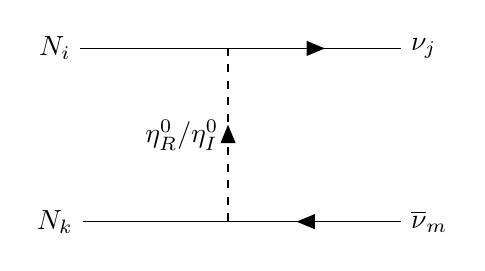
\begin{tikzpicture}
\begin{feynman}
\vertex (i1) {\(N_{i}\)};
\vertex[below=2.2cm of i1] (i2) {\(N_{k}\)};
\vertex[right=2.2cm of i1] (a);
\vertex[right=2.2cm of a] (f1) {\(\nu_{j}\)};
\vertex[below=2.2cm of a] (b);
\vertex[right=2.2cm of b] (f2) {\(\overline{\nu}_{m}\)};

\diagram*{
(i1) -- [plain] (a) -- [fermion] (f1),
(b) -- [charged scalar, edge label=\(\eta^{0}_R/\eta^{0}_I\)] (a),
(i2) -- [plain] b -- [anti fermion] (f2) [particle=\(N_{k}\)],
};
\end{feynman}
\end{tikzpicture}
}
%\hspace{1cm}
\subfigure[\(-h_{ij}\overline{l}_{i}\eta^{-}N_j + \hc\)]{
\begin{tikzpicture}
\begin{feynman}
\vertex (i1) {\(N_{i}\)};
\vertex[below=2.2cm of i1] (i2) {\(N_{k}\)};
\vertex[right=2.2cm of i1] (a);
\vertex[right=2.2cm of a] (f1) {\(l^{-}_{j}\)};
\vertex[below=2.2cm of a] (b);
\vertex[right=2.2cm of b] (f2) {\(l^{+}_{m}\)};

\diagram*{
(i1) -- [plain] (a) -- [fermion] (f1),
(b) -- [charged scalar, edge label=\(\eta^{\pm}\)] (a),
(i2) -- [plain] b -- [anti fermion] (f2),
};
\end{feynman}
\end{tikzpicture}
}
\caption{Fermionic singlet annihilation channels to leptons given by the scotogenic model}
\end{figure}
It is important to note that \(\eta\) could be in the bulk, and thus we may not just have one
particle, but an entire KK tower of states participating in the scalar propagator here; thus each of
these two channels is not unique, but rather there would be an infinite amount of channels per final
state, one for every \(\eta\) mass eigenstate, which would need to be summed over.  If we're talking
about DM, then we only ought to consider \(N_{1}\), these diagrams were left as general as possible
however.

Gravitons couple to the energy-momentum tensor, as it is the only other tensor a spin-2 field can
couple to. The energy-momentum tensor depends on the Lagrangian in its diagonal components.  This
means that interaction terms are included in such a tensor, thus they would couple with the graviton
field. Fermionic DM annihilation mediated by gravitons and radions would however not be different
when comparing my case with \cite{tfmfrancisco}, as the couplings I expect to find at tree level are
those of the graviton/radion with the fermionic DM's kinetic and mass terms.

\subsection{Is the extra scalar singlet in ScSM the radion?}
\label{sec:scsmrad}
The criteria I can think of off the top of my head are two; it needs to have the same quantum
numbers (so it must transform the same way) and (this is probably implied if the previous is met)
having the same couplings to fields.

Now, both are singlets under every symmetry bar scotogenic \(Z_{2}\); the radion is \(Z_{2}\)-even,
the scalar singlet is \(Z_{2}\)-odd. The latter \textit{has} to be odd, that is mostly its defining
characteristic. Thus, we should be ``molding'' the radion to the scalar singlet, rather.

\section{Dark matter}
\label{sec:darkmat}
\textbf{Requirements for a particle to be dark matter}: It has to be stable (very long lived, with lifetime
comparable to the age of the universe). Electrically neutral. A WIMP in particular is weakly interacting.

\section{Questions, answers, and musings}
\label{sec:qam}
Questions are in \textbf{bold}.
\begin{itemize}
\item Do we impose the VEV for the neutral part of the Higgs field? I'm asking because the parameters for
the Higgs field's potential seem, to me, to have the same parameters for the charged field and the
neutral field. How do we make the charged Higgs field to not have a non-zero VEV?

\item \textbf{How far down the rabbit hole should I go into needed concepts (orbifold, solving Einstein's field
equations in this configuration)?}
No need to get into those concepts at all.

\item \textbf{Why do we need boundary conditions to treat these two 3-branes?}
Distinguishing between even and odd field configurations.
Maybe also because geometric \(Z_2\) orbifold symmetry could be used as the \(Z_2\) scotogenic symmetry.

Extra dimensions were added to dark matter neutrinos in order to open up new decay (and production)
channels, since without them, the lack of right handed neutrinos would not explain observations.

\item In order to have the exponential factor in front of the regular part of the metric, one needs AdS.
(Empty spacetime negatively curved) That exponential factor is instrumental; it is what allows RS
to solve the hierarchy problem, its original purpose.

``Brane tension'' is just a term that can be written in the action, so it is added, it's a sort of
cosmological constant that is specific to the brane. The solution to the Einstein equations imposes
one tension to be negative and another positive. The cosmological constant of the bulk has to be negative.

\item \textbf{Why do we only consider two 3-branes?}
We need more than one because this introduces the hierarchy, and it is the most simple
setup beyond having just one. Also, consider that branes break translational invariance in
the fifth dimension. The mere fact that the physical region of the fifth dimension is smaller
than the periodicity (the physical region is ``half the circle'' given that everything is
mirrored in the other half, but the periodicity is over a ``whole circle'') also breaks
translational invariance. This means that momentum is not conserved along the fifth dimension,
as it is the generator of the translation transformation.

\item \textbf{What happens to the spacetime in between the branes?}
We just assume it has its own cosmological constant and that's it. Similarly, we just assume that
the hidden or UV brane has physics with a scale far above what we're looking for, thus they're
suppressed, which means that we don't take them into account. We do take into account its brane tension.

\item \textbf{What do we mean by ``stabilizing'' the size of the fifth dimension?}
These two branes have a Casimir attraction analog between them because the fifth dimension is
compactified (so modes are countably infinite and not uncountably infinite, it's just the same
principle), so \(r_c\) goes to 0 always. Branes act just like conductive plates; they act as borders to space.

\(kr_c\) has to have a concrete non-zero value; when one fixes the distance between branes, we get into a
problem because there is no justification for this. ``Stabilizing'' it means that there is an
additional field whose potential's minimum is related to \(r_c\) and sort of counteracts this Casimir effect.

\item \textbf{Where does the Majorana mass term for the RH neutrino come from? Is it put in by hand, or does it
have a dynamical origin like SM masses? Or should I not worry about this?}

\item \textbf{I take it I should handle the bulk fermion as if it were a Dirac fermion in the bulk,
but it somehow acquires a brane Majorana mass term, right?}

\item \textbf{On that note, it was outlined in \cite{Grossman_2000}, page 3, footnote 1 that a Dirac
fermion is chosen over a Majorana one because fermion number would be assigned to the bulk fermion.
Do we have a need for that here?} A possible answer is what is mentioned in \cite{Kadota_2008}, page
5, footnote 4; ``The Majorana spinors cannot exist in 5D because of the lack of the real
representation of gamma matrices but we can add the gauge- and Lorentz-invariant bilinear terms
for 5D Dirac isosinglet neutrino''

\item \textbf{Should I consider the hypothetical fourth sterile neutrino?}

\item If I understood correctly, I was only told to consider fermionic singlets to leptons, which probably
means that I would not be looking at all processes in order to calculate relic abundance,
rather this is for estimating the cross section of processes which are observable in particle
accelerators. Still, if that is the case, then I'd need to look at production channels as well.

Whatever I interpreted above however doesn't make a ton of sense because I imagine production cross
section is very low for these particles, thus there wouldn't be many and the chance of them
annihilating each other is \textit{very} low.

Going over the scope of this thesis, what should really be considered is the total annihilation
cross section, seeing how it increases by adding interactions with the radion and the graviton
while keeping the Yukawas around the same values, respecting LFV bounds.

\item The energy-momentum tensor depends on the Lagrangian in its diagonal components.
This means that interaction terms are included in such a tensor, thus they would couple with
the graviton field. Fermionic DM annihilation mediated by gravitons and radions would however
not be different when comparing my case with \cite{tfmfrancisco}, as the couplings I expect to
use at tree level are those of the graviton/radion with the fermionic DM's kinetic and mass terms.

\item The extra dimension is already finite before applying boundary conditions.

\item If \(\lambda_{5} = 0\), both self-energy diagrams yielding the mass matrix cancel each other
out completely, as \(m_{R} = m_{I}\). As such, there can be no lepton flavor violation, no lepton
flavor number violation and no mass matrix.
\end{itemize}

%2\Bigg[2 k \left(J_{\nu_{\eta}}\left(x_{n\nu_{\eta}}\right)
%-\frac{2J_{\nu}\left(x_{n\nu_{\eta}}\me^{-kr_c\pi}\right)
%+ x_{n\nu_{\eta}}\me^{-kr_c\pi}J'_{\nu}\left(x_{n\nu_{\eta}}\me^{-kr_c\pi}\right)}{2Y_{\nu}\left(x_{n\nu_{\eta}}\me^{-kr_c\pi}\right)
%+ x_{n\nu_{\eta}}\me^{-kr_c\pi}Y'_{\nu}\left(x_{n\nu_{\eta}}\me^{-kr_c\pi}\right)}
%Y_{\nu_{\eta}}\left(x_{n\nu_{\eta}}\right)\right) \\
%+ m_{\eta,n} \me^{kr_c\pi}\left(J'_{\nu_{\eta}}\left(x_{n\nu_{\eta}}\right)
%-\frac{2J_{\nu}\left(x_{n\nu_{\eta}}\me^{-kr_c\pi}\right)
%+ x_{n\nu_{\eta}}\me^{-kr_c\pi}J'_{\nu}\left(x_{n\nu_{\eta}}\me^{-kr_c\pi}\right)}{2Y_{\nu}\left(x_{n\nu_{\eta}}\me^{-kr_c\pi}\right)
%+ x_{n\nu_{\eta}}\me^{-kr_c\pi}Y'_{\nu}\left(x_{n\nu_{\eta}}\me^{-kr_c\pi}\right)}
%Y'_{\nu_{\eta}}\left(x_{n\nu_{\eta}}\right)\right)\Bigg] \\
%= - \frac{\lambda_3}{M_5} v^2_0 \Bigg[J_{\nu_{\eta}}\left(x_{n\nu_{\eta}}\right)
%-\frac{2J_{\nu}\left(x_{n\nu_{\eta}}\me^{-kr_c\pi}\right)
%+ x_{n\nu_{\eta}}\me^{-kr_c\pi}J'_{\nu}\left(x_{n\nu_{\eta}}\me^{-kr_c\pi}\right)}{2Y_{\nu}\left(x_{n\nu_{\eta}}\me^{-kr_c\pi}\right)
%+ x_{n\nu_{\eta}}\me^{-kr_c\pi}Y'_{\nu}\left(x_{n\nu_{\eta}}\me^{-kr_c\pi}\right)}
%Y_{\nu_{\eta}}\left(x_{n\nu_{\eta}}\right)\Bigg] \\
%\rightarrow

\appendix
\section{Notation and glossary}
\label{sec:not}
General, 4D spacetime indices are to be written with lower case Greek letters, starting with \(\mu\).
General, 5D spacetime indices are to be written with upper case Roman letters, starting with \(M\).
%Local, 4D spacetime indices are to be written with lower case Roman letters, starting with \(m\)
%Local, 5D spacetime indices are to be written with lower case Roman letters, starting with \(a\)
\begin{itemize}
\item SM: Standard Model
\item KK: Kaluza-Klein
\item RS: Randall-Sundrum
\item ScM: Scotogenic Model
\item ScSM: ScotoSinglet Model
\item GScM: Generalised Scotogenic Model
\item EWSB: ElectroWeak Symmetry Breaking

\item \(\Lambda\): Bulk (= 5D) cosmological constant
\item \(g/g_{\mathrm{IR}}\): 5D metric tensor determinant and the former, but evaluated at the IR brane
\item \(\varphi\): Variable representing the ``angle'' of the fifth dimensional ``circle''
\item \(f_{\mathrm{IR}}\), \(f_{\mathrm{UV}}\): Brane tensions (cosmological constants particular to branes)
\end{itemize}

\printbibliography

\end{document}